\documentclass[conference]{IEEEtran}

% Packages
\usepackage[utf8]{inputenc}
\usepackage[english]{babel}
\usepackage{amsmath}
\usepackage{amsfonts}
\usepackage{amssymb}
\usepackage{amsthm}
\usepackage{pdfpages}
\usepackage{graphicx}
\usepackage{epstopdf}
\usepackage{listings}
\usepackage{cite}
\usepackage{enumerate}
\usepackage{scientific}
\usepackage[colorlinks=false]{hyperref}
\usepackage{bookmark}

\usepackage[]{mcode}	%Matlab Code
\usepackage{tikz,pgfplots}	%Tikz

%\usepgfplotslibrary{external} 
%\tikzexternalize
%\tikzsetexternalprefix{ext/}

% Bookmark Setup
\bookmarksetup{numbered}

% PDF Setup
\hypersetup{pdftitle={Homework 6}, pdfsubject={Documentation of 6th Homework}, pdfauthor={Stefan Röhrl}, pdfkeywords={Neuroprothetik Exercise}, pdfcreator={LaTeX}, hidelinks}


\begin{document}
%
% cite all references
%\nocite{*}
%
% paper title
% can use linebreaks \\ within to get better formatting as desired
\title{Homework 6\\ Electric Stimulation}

\author{\IEEEauthorblockN{Stefan Röhrl}
\IEEEauthorblockA{Technische Universität München, Arcisstraße 21, Munich, Germany\\
Email: stefan.roehrl@tum.de}}

% use for special paper notices
%\IEEEspecialpapernotice{(Invited Paper)}

% make the title area
\maketitle

\IEEEpeerreviewmaketitle

\section{Calculate the Potential Field}

Das Potential auf einer der ebenen Fläche wird wie folgt berechnet:
\begin{lstlisting}
% Koordinaten in der X,Y-Ebene
[X,Y] =  meshgrid(-dim(1)/2:0.1:dim(1)/2,...
				  -dim(2)/2:0.1:dim(2)/2);
% Radialer Abstand
r = sqrt(X.^2 + Y.^2 + z^2);
% Potential
Phi = (rho_medium * I) ./ (4 * pi .* r);
\end{lstlisting}

\begin{enumerate}
\item Der Potenzialverlauf auf einer $50\mu m$ x $50\mu m$ Ebene über der eine Elektrode in $10\mu m$ Abstand angebracht ist in Abbildung \ref{fig:potField} dargestellt. Der Anregende Strom hat eine Größe von 1mA.

\begin{figure}[h]
	\centering
	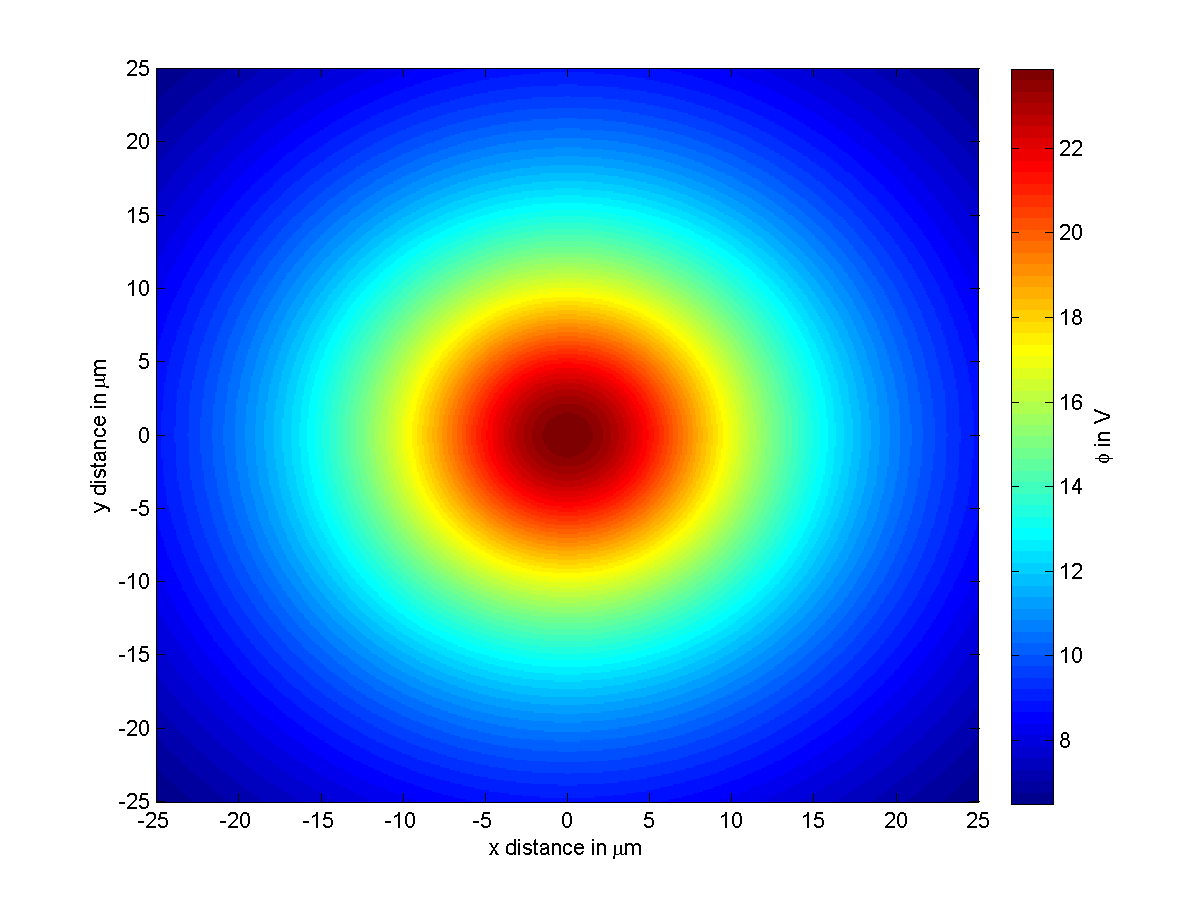
\includegraphics[width=0.5\textwidth]{img/potField.png}
	\caption{Potenzialfrei auf der Ebene}
	\label{fig:potField}
\end{figure}

\item Die folgenden drei Graphen zeigen den Potenzialverlauf (Abb. \ref{fig:Phi1}), das elektrische Feld (Abb. \ref{fig:E1}) und die Aktivierungsfunktion (Abb. \ref{fig:A1}) bei einem Elektrodenstrom von 1mA.\\

\begin{figure}[h!]
  	\centering
    \scalebox{.5}{% This file was created by matlab2tikz.
% Minimal pgfplots version: 1.3
%
%The latest updates can be retrieved from
%  http://www.mathworks.com/matlabcentral/fileexchange/22022-matlab2tikz
%where you can also make suggestions and rate matlab2tikz.
%
\begin{tikzpicture}

\begin{axis}[%
width=4.520833in,
height=3.565625in,
at={(0.758333in,0.48125in)},
scale only axis,
separate axis lines,
every outer x axis line/.append style={black},
every x tick label/.append style={font=\color{black}},
xmin=1,
xmax=501,
xtick={1,51,101,151,201,251,301,351,401,451,501},
xticklabels={{-25},{-20},{-15},{-10},{-5},{0},{5},{10},{15},{20},{25}},
xlabel={$\text{x distance in }\mu\text{m}$},
every outer y axis line/.append style={black},
every y tick label/.append style={font=\color{black}},
ymin=8,
ymax=24,
ylabel={$\phi\text{ in V}$},
title={$\phi\text{ with I = 1mA}$}
]
\addplot [color=blue,solid,forget plot]
  table[row sep=crcr]{%
1	8.86629929399968\\
2	8.8969700084153\\
3	8.92783637312795\\
4	8.95890006992601\\
5	8.99016279678701\\
6	9.02162626800457\\
7	9.0532922143142\\
8	9.08516238301814\\
9	9.11723853810915\\
10	9.14952246039295\\
11	9.18201594760935\\
12	9.2147208145518\\
13	9.24763889318544\\
14	9.28077203276323\\
15	9.31412209994021\\
16	9.34769097888575\\
17	9.38148057139342\\
18	9.41549279698855\\
19	9.4497295930332\\
20	9.48419291482831\\
21	9.51888473571293\\
22	9.55380704716026\\
23	9.58896185887038\\
24	9.62435119885929\\
25	9.65997711354423\\
26	9.69584166782492\\
27	9.73194694516044\\
28	9.76829504764166\\
29	9.80488809605876\\
30	9.84172822996365\\
31	9.87881760772705\\
32	9.91615840658981\\
33	9.95375282270821\\
34	9.99160307119295\\
35	10.0297113861414\\
36	10.0680800206629\\
37	10.1067112468965\\
38	10.1456073560207\\
39	10.1847706582558\\
40	10.2242034828564\\
41	10.2639081780958\\
42	10.3038871112406\\
43	10.3441426685148\\
44	10.3846772550542\\
45	10.4254932948493\\
46	10.4665932306765\\
47	10.5079795240181\\
48	10.5496546549681\\
49	10.5916211221265\\
50	10.633881442478\\
51	10.6764381512577\\
52	10.7192938018002\\
53	10.762450965374\\
54	10.8059122309984\\
55	10.8496802052432\\
56	10.8937575120104\\
57	10.9381467922972\\
58	10.9828507039382\\
59	11.0278719213278\\
60	11.0732131351206\\
61	11.1188770519094\\
62	11.1648663938792\\
63	11.2111838984375\\
64	11.257832317818\\
65	11.3048144186584\\
66	11.3521329815496\\
67	11.3997908005568\\
68	11.4477906827095\\
69	11.4961354474605\\
70	11.5448279261121\\
71	11.5938709612075\\
72	11.6432674058876\\
73	11.6930201232103\\
74	11.743131985431\\
75	11.7936058732433\\
76	11.8444446749783\\
77	11.8956512857599\\
78	11.9472286066156\\
79	11.9991795435399\\
80	12.0515070065092\\
81	12.1042139084464\\
82	12.1573031641322\\
83	12.2107776890623\\
84	12.2646403982476\\
85	12.3188942049555\\
86	12.3735420193902\\
87	12.4285867473089\\
88	12.4840312885732\\
89	12.5398785356309\\
90	12.5961313719278\\
91	12.6527926702456\\
92	12.7098652909639\\
93	12.7673520802425\\
94	12.8252558681227\\
95	12.8835794665432\\
96	12.9423256672684\\
97	13.0014972397258\\
98	13.061096928749\\
99	13.1211274522235\\
100	13.1815914986317\\
101	13.2424917244934\\
102	13.3038307516985\\
103	13.3656111647286\\
104	13.4278355077628\\
105	13.4905062816651\\
106	13.5536259408487\\
107	13.6171968900131\\
108	13.6812214807503\\
109	13.7457020080167\\
110	13.8106407064644\\
111	13.8760397466298\\
112	13.9419012309738\\
113	14.0082271897692\\
114	14.0750195768319\\
115	14.1422802650897\\
116	14.2100110419851\\
117	14.2782136047073\\
118	14.3468895552481\\
119	14.4160403952782\\
120	14.4856675208368\\
121	14.5557722168323\\
122	14.6263556513477\\
123	14.6974188697452\\
124	14.7689627885681\\
125	14.8409881892309\\
126	14.913495711497\\
127	14.9864858467361\\
128	15.0599589309589\\
129	15.1339151376226\\
130	15.2083544702045\\
131	15.2832767545379\\
132	15.3586816309074\\
133	15.434568545898\\
134	15.5109367439959\\
135	15.5877852589363\\
136	15.6651129047951\\
137	15.7429182668212\\
138	15.8211996920078\\
139	15.8999552793983\\
140	15.9791828701272\\
141	16.0588800371924\\
142	16.1390440749589\\
143	16.2196719883934\\
144	16.3007604820292\\
145	16.3823059486627\\
146	16.4643044577823\\
147	16.5467517437324\\
148	16.6296431936146\\
149	16.7129738349299\\
150	16.7967383229679\\
151	16.8809309279457\\
152	16.9655455219068\\
153	17.050575565384\\
154	17.1360140938388\\
155	17.2218537038844\\
156	17.3080865393063\\
157	17.3947042768919\\
158	17.4816981120845\\
159	17.5690587444772\\
160	17.6567763631654\\
161	17.744840631976\\
162	17.833240674596\\
163	17.9219650596237\\
164	18.0110017855666\\
165	18.1003382658155\\
166	18.1899613136226\\
167	18.2798571271167\\
168	18.370011274389\\
169	18.4604086786875\\
170	18.5510336037574\\
171	18.6418696393712\\
172	18.7328996870913\\
173	18.8241059463135\\
174	18.9154699006402\\
175	19.0069723046371\\
176	19.0985931710274\\
177	19.1903117583826\\
178	19.2821065593705\\
179	19.3739552896247\\
180	19.465834877301\\
181	19.5577214533908\\
182	19.649590342863\\
183	19.7414160567084\\
184	19.8331722849637\\
185	19.9248318907938\\
186	20.0163669057136\\
187	20.1077485260321\\
188	20.1989471106031\\
189	20.2899321799699\\
190	20.3806724169889\\
191	20.4711356690224\\
192	20.5612889517878\\
193	20.6510984549515\\
194	20.7405295495568\\
195	20.8295467973721\\
196	20.9181139622468\\
197	21.0061940235573\\
198	21.0937491918274\\
199	21.1807409265998\\
200	21.2671299566362\\
201	21.3528763025153\\
202	21.4379393016965\\
203	21.5222776361092\\
204	21.6058493623217\\
205	21.6886119443383\\
206	21.7705222890629\\
207	21.8515367844602\\
208	21.9316113404367\\
209	22.0107014324528\\
210	22.0887621478666\\
211	22.1657482349992\\
212	22.2416141548987\\
213	22.3163141357665\\
214	22.3898022299986\\
215	22.4620323737772\\
216	22.5329584491365\\
217	22.6025343484108\\
218	22.6707140409568\\
219	22.7374516420283\\
220	22.8027014836653\\
221	22.8664181874441\\
222	22.9285567389191\\
223	22.989072563573\\
224	23.0479216040761\\
225	23.1050603986414\\
226	23.1604461602489\\
227	23.2140368564986\\
228	23.2657912898409\\
229	23.3156691779195\\
230	23.3636312337557\\
231	23.4096392454901\\
232	23.4536561553939\\
233	23.4956461378539\\
234	23.5355746760321\\
235	23.5734086368993\\
236	23.6091163443391\\
237	23.6426676500222\\
238	23.6740340017532\\
239	23.7031885089971\\
240	23.7301060053\\
241	23.7547631073285\\
242	23.7771382702615\\
243	23.7972118392823\\
244	23.8149660969353\\
245	23.830385306124\\
246	23.8434557485501\\
247	23.85416575841\\
248	23.8625057511884\\
249	23.8684682474087\\
250	23.8720478912283\\
251	23.8732414637843\\
252	23.8720478912283\\
253	23.8684682474087\\
254	23.8625057511884\\
255	23.85416575841\\
256	23.8434557485501\\
257	23.830385306124\\
258	23.8149660969353\\
259	23.7972118392823\\
260	23.7771382702615\\
261	23.7547631073285\\
262	23.7301060053\\
263	23.7031885089971\\
264	23.6740340017532\\
265	23.6426676500222\\
266	23.6091163443391\\
267	23.5734086368993\\
268	23.5355746760321\\
269	23.4956461378539\\
270	23.4536561553939\\
271	23.4096392454901\\
272	23.3636312337557\\
273	23.3156691779195\\
274	23.2657912898409\\
275	23.2140368564986\\
276	23.1604461602489\\
277	23.1050603986414\\
278	23.0479216040761\\
279	22.989072563573\\
280	22.9285567389191\\
281	22.8664181874441\\
282	22.8027014836653\\
283	22.7374516420283\\
284	22.6707140409568\\
285	22.6025343484108\\
286	22.5329584491365\\
287	22.4620323737772\\
288	22.3898022299986\\
289	22.3163141357665\\
290	22.2416141548987\\
291	22.1657482349992\\
292	22.0887621478666\\
293	22.0107014324528\\
294	21.9316113404367\\
295	21.8515367844602\\
296	21.7705222890629\\
297	21.6886119443383\\
298	21.6058493623217\\
299	21.5222776361092\\
300	21.4379393016965\\
301	21.3528763025153\\
302	21.2671299566362\\
303	21.1807409265998\\
304	21.0937491918274\\
305	21.0061940235573\\
306	20.9181139622468\\
307	20.8295467973721\\
308	20.7405295495568\\
309	20.6510984549515\\
310	20.5612889517878\\
311	20.4711356690224\\
312	20.3806724169889\\
313	20.2899321799699\\
314	20.1989471106031\\
315	20.1077485260321\\
316	20.0163669057136\\
317	19.9248318907938\\
318	19.8331722849637\\
319	19.7414160567084\\
320	19.649590342863\\
321	19.5577214533908\\
322	19.465834877301\\
323	19.3739552896247\\
324	19.2821065593705\\
325	19.1903117583826\\
326	19.0985931710274\\
327	19.0069723046371\\
328	18.9154699006402\\
329	18.8241059463135\\
330	18.7328996870913\\
331	18.6418696393712\\
332	18.5510336037574\\
333	18.4604086786875\\
334	18.370011274389\\
335	18.2798571271167\\
336	18.1899613136226\\
337	18.1003382658155\\
338	18.0110017855666\\
339	17.9219650596237\\
340	17.833240674596\\
341	17.744840631976\\
342	17.6567763631654\\
343	17.5690587444772\\
344	17.4816981120845\\
345	17.3947042768919\\
346	17.3080865393063\\
347	17.2218537038844\\
348	17.1360140938388\\
349	17.050575565384\\
350	16.9655455219068\\
351	16.8809309279457\\
352	16.7967383229679\\
353	16.7129738349299\\
354	16.6296431936146\\
355	16.5467517437324\\
356	16.4643044577823\\
357	16.3823059486627\\
358	16.3007604820292\\
359	16.2196719883934\\
360	16.1390440749589\\
361	16.0588800371924\\
362	15.9791828701272\\
363	15.8999552793983\\
364	15.8211996920078\\
365	15.7429182668212\\
366	15.6651129047951\\
367	15.5877852589363\\
368	15.5109367439959\\
369	15.434568545898\\
370	15.3586816309074\\
371	15.2832767545379\\
372	15.2083544702045\\
373	15.1339151376226\\
374	15.0599589309589\\
375	14.9864858467361\\
376	14.913495711497\\
377	14.8409881892309\\
378	14.7689627885681\\
379	14.6974188697452\\
380	14.6263556513477\\
381	14.5557722168323\\
382	14.4856675208368\\
383	14.4160403952782\\
384	14.3468895552481\\
385	14.2782136047073\\
386	14.2100110419851\\
387	14.1422802650897\\
388	14.0750195768319\\
389	14.0082271897692\\
390	13.9419012309738\\
391	13.8760397466298\\
392	13.8106407064644\\
393	13.7457020080167\\
394	13.6812214807503\\
395	13.6171968900131\\
396	13.5536259408487\\
397	13.4905062816651\\
398	13.4278355077628\\
399	13.3656111647286\\
400	13.3038307516985\\
401	13.2424917244934\\
402	13.1815914986317\\
403	13.1211274522235\\
404	13.061096928749\\
405	13.0014972397258\\
406	12.9423256672684\\
407	12.8835794665432\\
408	12.8252558681227\\
409	12.7673520802425\\
410	12.7098652909639\\
411	12.6527926702456\\
412	12.5961313719278\\
413	12.5398785356309\\
414	12.4840312885732\\
415	12.4285867473089\\
416	12.3735420193902\\
417	12.3188942049555\\
418	12.2646403982476\\
419	12.2107776890623\\
420	12.1573031641322\\
421	12.1042139084464\\
422	12.0515070065092\\
423	11.9991795435399\\
424	11.9472286066156\\
425	11.8956512857599\\
426	11.8444446749783\\
427	11.7936058732433\\
428	11.743131985431\\
429	11.6930201232103\\
430	11.6432674058876\\
431	11.5938709612075\\
432	11.5448279261121\\
433	11.4961354474605\\
434	11.4477906827095\\
435	11.3997908005568\\
436	11.3521329815496\\
437	11.3048144186584\\
438	11.257832317818\\
439	11.2111838984375\\
440	11.1648663938792\\
441	11.1188770519094\\
442	11.0732131351206\\
443	11.0278719213278\\
444	10.9828507039382\\
445	10.9381467922972\\
446	10.8937575120104\\
447	10.8496802052432\\
448	10.8059122309984\\
449	10.762450965374\\
450	10.7192938018002\\
451	10.6764381512577\\
452	10.633881442478\\
453	10.5916211221265\\
454	10.5496546549681\\
455	10.5079795240181\\
456	10.4665932306765\\
457	10.4254932948493\\
458	10.3846772550542\\
459	10.3441426685148\\
460	10.3038871112406\\
461	10.2639081780958\\
462	10.2242034828564\\
463	10.1847706582558\\
464	10.1456073560207\\
465	10.1067112468965\\
466	10.0680800206629\\
467	10.0297113861414\\
468	9.99160307119295\\
469	9.95375282270821\\
470	9.91615840658981\\
471	9.87881760772705\\
472	9.84172822996365\\
473	9.80488809605876\\
474	9.76829504764166\\
475	9.73194694516044\\
476	9.69584166782492\\
477	9.65997711354423\\
478	9.62435119885929\\
479	9.58896185887038\\
480	9.55380704716026\\
481	9.51888473571293\\
482	9.48419291482831\\
483	9.4497295930332\\
484	9.41549279698855\\
485	9.38148057139342\\
486	9.34769097888575\\
487	9.31412209994021\\
488	9.28077203276323\\
489	9.24763889318544\\
490	9.2147208145518\\
491	9.18201594760935\\
492	9.14952246039295\\
493	9.11723853810915\\
494	9.08516238301814\\
495	9.0532922143142\\
496	9.02162626800457\\
497	8.99016279678701\\
498	8.95890006992601\\
499	8.92783637312795\\
500	8.8969700084153\\
501	8.86629929399968\\
};
\end{axis}
\end{tikzpicture}%}
    \vspace{-10pt}
    \caption{Potenzialverlauf im Axon bei I = 1mA}
    \vspace{-10pt}
    \label{fig:Phi1}
\end{figure}
\begin{figure}[h!]
  	\centering
    \scalebox{.5}{% This file was created by matlab2tikz.
% Minimal pgfplots version: 1.3
%
%The latest updates can be retrieved from
%  http://www.mathworks.com/matlabcentral/fileexchange/22022-matlab2tikz
%where you can also make suggestions and rate matlab2tikz.
%
\begin{tikzpicture}

\begin{axis}[%
width=4.520833in,
height=3.565625in,
at={(0.758333in,0.48125in)},
scale only axis,
separate axis lines,
every outer x axis line/.append style={black},
every x tick label/.append style={font=\color{black}},
xmin=1,
xmax=501,
xtick={1,51,101,151,201,251,301,351,401,451,501},
xticklabels={{-25},{-20},{-15},{-10},{-5},{0},{5},{10},{15},{20},{25}},
xlabel={$\text{x distance in }\mu\text{m}$},
every outer y axis line/.append style={black},
every y tick label/.append style={font=\color{black}},
ymin=-1,
ymax=1,
ylabel={$\text{E in V/}\mu\text{m}$},
title={E with I = 1mA}
]
\addplot [color=blue,solid,forget plot]
  table[row sep=crcr]{%
1	-0.306707144156118\\
2	-0.308663647126579\\
3	-0.310636967980518\\
4	-0.312627268610068\\
5	-0.314634712175614\\
6	-0.316659463096229\\
7	-0.318701687039393\\
8	-0.32076155091012\\
9	-0.322839222838027\\
10	-0.32493487216394\\
11	-0.327048669424581\\
12	-0.329180786336387\\
13	-0.331331395777834\\
14	-0.333500671769862\\
15	-0.335688789455411\\
16	-0.337895925076648\\
17	-0.340122255951325\\
18	-0.342367960446506\\
19	-0.344633217951085\\
20	-0.346918208846176\\
21	-0.349223114473336\\
22	-0.351548117101199\\
23	-0.353893399889067\\
24	-0.35625914684946\\
25	-0.358645542806855\\
26	-0.361052773355208\\
27	-0.363481024812238\\
28	-0.36593048417096\\
29	-0.368401339048887\\
30	-0.370893777634009\\
31	-0.373407988627594\\
32	-0.37594416118397\\
33	-0.378502484847481\\
34	-0.381083149484756\\
35	-0.383686345215093\\
36	-0.38631226233532\\
37	-0.388961091242361\\
38	-0.39163302235071\\
39	-0.394328246006062\\
40	-0.39704695239454\\
41	-0.399789331447735\\
42	-0.402555572741985\\
43	-0.405345865394047\\
44	-0.408160397950539\\
45	-0.410999358272743\\
46	-0.413862933415476\\
47	-0.416751309500434\\
48	-0.419664671583373\\
49	-0.422603203515255\\
50	-0.425567087796601\\
51	-0.428556505425508\\
52	-0.431571635738397\\
53	-0.434612656243658\\
54	-0.437679742447603\\
55	-0.440773067672762\\
56	-0.443892802867989\\
57	-0.447039116409851\\
58	-0.450212173895892\\
59	-0.453412137928133\\
60	-0.456639167887527\\
61	-0.459893419698432\\
62	-0.463175045582975\\
63	-0.466484193805172\\
64	-0.469821008403297\\
65	-0.473185628912027\\
66	-0.47657819007199\\
67	-0.479998821527143\\
68	-0.483447647510538\\
69	-0.486924786515335\\
70	-0.490430350953872\\
71	-0.493964446801574\\
72	-0.497527173227006\\
73	-0.501118622206533\\
74	-0.50473887812311\\
75	-0.508388017350008\\
76	-0.512066107816427\\
77	-0.515773208556922\\
78	-0.519509369242517\\
79	-0.52327462969318\\
80	-0.527069019371833\\
81	-0.530892556857978\\
82	-0.534745249301025\\
83	-0.538627091853066\\
84	-0.542538067079441\\
85	-0.546478144346541\\
86	-0.550447279187516\\
87	-0.554445412642739\\
88	-0.558472470576685\\
89	-0.562528362968973\\
90	-0.566612983178718\\
91	-0.570726207182872\\
92	-0.57486789278606\\
93	-0.579037878801802\\
94	-0.58323598420472\\
95	-0.587462007251975\\
96	-0.591715724573767\\
97	-0.595996890231945\\
98	-0.600305234745502\\
99	-0.604640464082369\\
100	-0.609002258616833\\
101	-0.613390272051006\\
102	-0.617804130300428\\
103	-0.6222434303419\\
104	-0.626707739023669\\
105	-0.631196591836165\\
106	-0.63570949164319\\
107	-0.640245907372314\\
108	-0.644805272663849\\
109	-0.649386984477172\\
110	-0.653990401654259\\
111	-0.658614843439498\\
112	-0.663259587954386\\
113	-0.667923870627352\\
114	-0.672606882577984\\
115	-0.67730776895381\\
116	-0.682025627221385\\
117	-0.686759505408663\\
118	-0.69150840030062\\
119	-0.696271255585952\\
120	-0.701046959955587\\
121	-0.705834345153065\\
122	-0.710632183975815\\
123	-0.715439188228579\\
124	-0.720254006628203\\
125	-0.725075222660738\\
126	-0.729901352391416\\
127	-0.734730842227727\\
128	-0.739562066636967\\
129	-0.744393325818713\\
130	-0.749222843334518\\
131	-0.754048763694684\\
132	-0.758869149905763\\
133	-0.763681980979314\\
134	-0.768485149404494\\
135	-0.773276458587677\\
136	-0.778053620261314\\
137	-0.782814251865371\\
138	-0.787555873905088\\
139	-0.792275907289213\\
140	-0.796971670651878\\
141	-0.801640377665152\\
142	-0.806279134344869\\
143	-0.810884936357859\\
144	-0.81545466633461\\
145	-0.819985091196251\\
146	-0.824472859501348\\
147	-0.82891449882144\\
148	-0.833306413153778\\
149	-0.8376448803795\\
150	-0.841926049778579\\
151	-0.846145939610352\\
152	-0.850300434772322\\
153	-0.854385284547767\\
154	-0.858396100456034\\
155	-0.862328354218995\\
156	-0.866177375856125\\
157	-0.869938351925796\\
158	-0.87360632392766\\
159	-0.877176186882025\\
160	-0.880642688105553\\
161	-0.884000426200195\\
162	-0.887243850276391\\
163	-0.890367259429148\\
164	-0.893364802489351\\
165	-0.896230478071338\\
166	-0.898958134940528\\
167	-0.901541472723153\\
168	-0.90397404298475\\
169	-0.90624925069946\\
170	-0.908360356137976\\
171	-0.910300477200998\\
172	-0.912062592221332\\
173	-0.913639543267308\\
174	-0.915024039969445\\
175	-0.916208663903006\\
176	-0.91718587355146\\
177	-0.917948009879126\\
178	-0.918487302542061\\
179	-0.91879587676285\\
180	-0.918865760898129\\
181	-0.918688894721882\\
182	-0.918257138453811\\
183	-0.917562282552922\\
184	-0.916596058301238\\
185	-0.915350149198311\\
186	-0.913816203184545\\
187	-0.911985845710355\\
188	-0.909850693667522\\
189	-0.907402370189878\\
190	-0.904632520335689\\
191	-0.901532827654208\\
192	-0.898095031636927\\
193	-0.894310946052315\\
194	-0.890172478153417\\
195	-0.885671648746609\\
196	-0.88080061310535\\
197	-0.875551682700753\\
198	-0.86991734772436\\
199	-0.863890300363934\\
200	-0.857463458791052\\
201	-0.850629991812362\\
202	-0.843383344126423\\
203	-0.83571726212476\\
204	-0.827625820166595\\
205	-0.819103447246157\\
206	-0.810144953973015\\
207	-0.800745559765019\\
208	-0.790900920160738\\
209	-0.780607154137627\\
210	-0.769860871326351\\
211	-0.7586591989946\\
212	-0.746999808678481\\
213	-0.734880942321112\\
214	-0.722301437785546\\
215	-0.709260753593099\\
216	-0.695758992743407\\
217	-0.681796925459963\\
218	-0.667376010714733\\
219	-0.652498416369944\\
220	-0.637167037787734\\
221	-0.621385514749981\\
222	-0.605158246539297\\
223	-0.588490405031195\\
224	-0.57138794565315\\
225	-0.553857616074644\\
226	-0.535906962497315\\
227	-0.517544333422322\\
228	-0.498778880785942\\
229	-0.479620558361908\\
230	-0.460080117344503\\
231	-0.440169099038421\\
232	-0.419899824599383\\
233	-0.399285381781773\\
234	-0.378339608672036\\
235	-0.357077074397942\\
236	-0.335513056831296\\
237	-0.31366351731009\\
238	-0.291545072438595\\
239	-0.269174963029286\\
240	-0.246571020285558\\
241	-0.223751629329243\\
242	-0.200735690208518\\
243	-0.177542576530065\\
244	-0.154192091887033\\
245	-0.130704424260806\\
246	-0.107100098599382\\
247	-0.0833999277830344\\
248	-0.0596249622038414\\
249	-0.0357964381957387\\
250	-0.0119357255599439\\
251	0.0119357255599439\\
252	0.0357964381957387\\
253	0.0596249622038414\\
254	0.0833999277830344\\
255	0.107100098599382\\
256	0.130704424260806\\
257	0.154192091887033\\
258	0.177542576530065\\
259	0.200735690208518\\
260	0.223751629329243\\
261	0.246571020285558\\
262	0.269174963029286\\
263	0.291545072438595\\
264	0.31366351731009\\
265	0.335513056831296\\
266	0.357077074397942\\
267	0.378339608672036\\
268	0.399285381781773\\
269	0.419899824599383\\
270	0.440169099038421\\
271	0.460080117344503\\
272	0.479620558361908\\
273	0.498778880785942\\
274	0.517544333422322\\
275	0.535906962497315\\
276	0.553857616074644\\
277	0.57138794565315\\
278	0.588490405031195\\
279	0.605158246539297\\
280	0.621385514749981\\
281	0.637167037787734\\
282	0.652498416369944\\
283	0.667376010714733\\
284	0.681796925459963\\
285	0.695758992743407\\
286	0.709260753593099\\
287	0.722301437785546\\
288	0.734880942321112\\
289	0.746999808678481\\
290	0.7586591989946\\
291	0.769860871326351\\
292	0.780607154137627\\
293	0.790900920160738\\
294	0.800745559765019\\
295	0.810144953973015\\
296	0.819103447246157\\
297	0.827625820166595\\
298	0.83571726212476\\
299	0.843383344126423\\
300	0.850629991812362\\
301	0.857463458791052\\
302	0.863890300363934\\
303	0.86991734772436\\
304	0.875551682700753\\
305	0.88080061310535\\
306	0.885671648746609\\
307	0.890172478153417\\
308	0.894310946052315\\
309	0.898095031636927\\
310	0.901532827654208\\
311	0.904632520335689\\
312	0.907402370189878\\
313	0.909850693667522\\
314	0.911985845710355\\
315	0.913816203184545\\
316	0.915350149198311\\
317	0.916596058301238\\
318	0.917562282552922\\
319	0.918257138453811\\
320	0.918688894721882\\
321	0.918865760898129\\
322	0.91879587676285\\
323	0.918487302542061\\
324	0.917948009879126\\
325	0.91718587355146\\
326	0.916208663903006\\
327	0.915024039969445\\
328	0.913639543267308\\
329	0.912062592221332\\
330	0.910300477200998\\
331	0.908360356137976\\
332	0.90624925069946\\
333	0.90397404298475\\
334	0.901541472723153\\
335	0.898958134940528\\
336	0.896230478071338\\
337	0.893364802489351\\
338	0.890367259429148\\
339	0.887243850276391\\
340	0.884000426200195\\
341	0.880642688105553\\
342	0.877176186882025\\
343	0.87360632392766\\
344	0.869938351925796\\
345	0.866177375856125\\
346	0.862328354218995\\
347	0.858396100456034\\
348	0.854385284547767\\
349	0.850300434772322\\
350	0.846145939610352\\
351	0.841926049778579\\
352	0.8376448803795\\
353	0.833306413153778\\
354	0.82891449882144\\
355	0.824472859501348\\
356	0.819985091196251\\
357	0.81545466633461\\
358	0.810884936357859\\
359	0.806279134344869\\
360	0.801640377665152\\
361	0.796971670651878\\
362	0.792275907289213\\
363	0.787555873905088\\
364	0.782814251865371\\
365	0.778053620261314\\
366	0.773276458587677\\
367	0.768485149404494\\
368	0.763681980979314\\
369	0.758869149905763\\
370	0.754048763694684\\
371	0.749222843334518\\
372	0.744393325818713\\
373	0.739562066636967\\
374	0.734730842227727\\
375	0.729901352391416\\
376	0.725075222660738\\
377	0.720254006628203\\
378	0.715439188228579\\
379	0.710632183975815\\
380	0.705834345153065\\
381	0.701046959955587\\
382	0.696271255585952\\
383	0.69150840030062\\
384	0.686759505408663\\
385	0.682025627221385\\
386	0.67730776895381\\
387	0.672606882577984\\
388	0.667923870627352\\
389	0.663259587954386\\
390	0.658614843439498\\
391	0.653990401654259\\
392	0.649386984477172\\
393	0.644805272663849\\
394	0.640245907372314\\
395	0.63570949164319\\
396	0.631196591836165\\
397	0.626707739023669\\
398	0.6222434303419\\
399	0.617804130300428\\
400	0.613390272051006\\
401	0.609002258616833\\
402	0.604640464082369\\
403	0.600305234745502\\
404	0.595996890231945\\
405	0.591715724573767\\
406	0.587462007251975\\
407	0.58323598420472\\
408	0.579037878801802\\
409	0.57486789278606\\
410	0.570726207182872\\
411	0.566612983178718\\
412	0.562528362968973\\
413	0.558472470576685\\
414	0.554445412642739\\
415	0.550447279187516\\
416	0.546478144346541\\
417	0.542538067079441\\
418	0.538627091853066\\
419	0.534745249301025\\
420	0.530892556857978\\
421	0.527069019371833\\
422	0.52327462969318\\
423	0.519509369242517\\
424	0.515773208556922\\
425	0.512066107816427\\
426	0.508388017350008\\
427	0.50473887812311\\
428	0.501118622206533\\
429	0.497527173227006\\
430	0.493964446801574\\
431	0.490430350953872\\
432	0.486924786515335\\
433	0.483447647510538\\
434	0.479998821527143\\
435	0.47657819007199\\
436	0.473185628912027\\
437	0.469821008403297\\
438	0.466484193805172\\
439	0.463175045582975\\
440	0.459893419698432\\
441	0.456639167887527\\
442	0.453412137928133\\
443	0.450212173895892\\
444	0.447039116409851\\
445	0.443892802867989\\
446	0.440773067672762\\
447	0.437679742447603\\
448	0.434612656243658\\
449	0.431571635738397\\
450	0.428556505425508\\
451	0.425567087796601\\
452	0.422603203515255\\
453	0.419664671583373\\
454	0.416751309500434\\
455	0.413862933415476\\
456	0.410999358272743\\
457	0.408160397950539\\
458	0.405345865394047\\
459	0.402555572741985\\
460	0.399789331447735\\
461	0.39704695239454\\
462	0.394328246006062\\
463	0.39163302235071\\
464	0.388961091242361\\
465	0.38631226233532\\
466	0.383686345215093\\
467	0.381083149484756\\
468	0.378502484847481\\
469	0.37594416118397\\
470	0.373407988627594\\
471	0.370893777634009\\
472	0.368401339048887\\
473	0.36593048417096\\
474	0.363481024812238\\
475	0.361052773355208\\
476	0.358645542806855\\
477	0.35625914684946\\
478	0.353893399889067\\
479	0.351548117101199\\
480	0.349223114473336\\
481	0.346918208846176\\
482	0.344633217951085\\
483	0.342367960446506\\
484	0.340122255951325\\
485	0.337895925076648\\
486	0.335688789455411\\
487	0.333500671769862\\
488	0.331331395777834\\
489	0.329180786336387\\
490	0.327048669424581\\
491	0.32493487216394\\
492	0.322839222838027\\
493	0.32076155091012\\
494	0.318701687039393\\
495	0.316659463096229\\
496	0.314634712175614\\
497	0.312627268610068\\
498	0.310636967980518\\
499	0.308663647126579\\
500	0.306707144156118\\
501	0.306707144156118\\
};
\end{axis}
\end{tikzpicture}%}
    \vspace{-10pt}
    \caption{Elektrisches Feld im Axon bei I = 1mA}
    \vspace{-10pt}
    \label{fig:E1}
\end{figure}
\begin{figure}[h!]
  	\centering
    \scalebox{.5}{% This file was created by matlab2tikz.
% Minimal pgfplots version: 1.3
%
%The latest updates can be retrieved from
%  http://www.mathworks.com/matlabcentral/fileexchange/22022-matlab2tikz
%where you can also make suggestions and rate matlab2tikz.
%
\begin{tikzpicture}

\begin{axis}[%
width=4.520833in,
height=3.565625in,
at={(0.758333in,0.48125in)},
scale only axis,
separate axis lines,
every outer x axis line/.append style={black},
every x tick label/.append style={font=\color{black}},
xmin=1,
xmax=501,
xtick={1,51,101,151,201,251,301,351,401,451,501},
xticklabels={{-25},{-20},{-15},{-10},{-5},{0},{5},{10},{15},{20},{25}},
xlabel={$\text{x distance in }\mu\text{m}$},
every outer y axis line/.append style={black},
every y tick label/.append style={font=\color{black}},
ymin=-250,
ymax=50,
ylabel={$\text{Activationfunction in mV/ }\mu\text{m}^\text{2}$},
title={Activation with I = 1mA}
]
\addplot [color=blue,solid,forget plot]
  table[row sep=crcr]{%
1	19.5650297047905\\
2	19.733208539219\\
3	19.9030062954989\\
4	20.0744356554424\\
5	20.2475092060922\\
6	20.4222394317185\\
7	20.5986387072699\\
8	20.7767192790925\\
9	20.9564932591093\\
10	21.1379726064479\\
11	21.3211691179822\\
12	21.506094414508\\
13	21.69275992037\\
14	21.8811768552769\\
15	22.0713562126548\\
16	22.263308746551\\
17	22.4570449518069\\
18	22.6525750458677\\
19	22.8499089509569\\
20	23.0490562715204\\
21	23.2500262785834\\
22	23.4528278788275\\
23	23.6574696038588\\
24	23.8639595738277\\
25	24.0723054837872\\
26	24.2825145700408\\
27	24.4945935874057\\
28	24.7085487791992\\
29	24.9243858512273\\
30	25.1421099357685\\
31	25.3617255639256\\
32	25.5832366348841\\
33	25.8066463729847\\
34	26.0319573031666\\
35	26.2591712024005\\
36	26.488289070403\\
37	26.7193110834341\\
38	26.9522365535522\\
39	27.1870638847758\\
40	27.4237905319751\\
41	27.6624129424817\\
42	27.9029265206191\\
43	28.1453255649467\\
44	28.3896032220582\\
45	28.6357514272822\\
46	28.8837608495669\\
47	29.1336208294524\\
48	29.3853193186806\\
49	29.6388428136197\\
50	29.8941762888717\\
51	30.1513031290597\\
52	30.4102050526126\\
53	30.6708620393692\\
54	30.9332522516343\\
55	31.1973519523235\\
56	31.4631354185622\\
57	31.7305748603758\\
58	31.999640322465\\
59	32.2702995939835\\
60	32.5425181088576\\
61	32.8162588455598\\
62	33.0914822219711\\
63	33.3681459813306\\
64	33.6462050872797\\
65	33.9256115994431\\
66	34.2063145517386\\
67	34.488259833779\\
68	34.7713900480812\\
69	35.0556443852838\\
70	35.3409584771725\\
71	35.6272642542535\\
72	35.914489795141\\
73	36.2025591659403\\
74	36.4913922689084\\
75	36.7809046641923\\
76	37.0710074050294\\
77	37.3616068558476\\
78	37.6526045065475\\
79	37.9438967867827\\
80	38.2353748611422\\
81	38.5269244306983\\
82	38.8184255203669\\
83	39.109752263721\\
84	39.4007726710697\\
85	39.6913484095421\\
86	39.9813345524308\\
87	40.2705793394489\\
88	40.5589239227993\\
89	40.8462020974184\\
90	41.1322400417703\\
91	41.4168560317194\\
92	41.6998601573141\\
93	41.9810540293838\\
94	42.2602304723114\\
95	42.5371732180793\\
96	42.8116565817618\\
97	43.0834451355622\\
98	43.3522933686618\\
99	43.6179453447039\\
100	43.8801343416344\\
101	44.1385824942699\\
102	44.3930004148569\\
103	44.6430868174502\\
104	44.8885281250114\\
105	45.1289980703223\\
106	45.3641572912602\\
107	45.5936529153405\\
108	45.8171181331636\\
109	46.0341717709525\\
110	46.2444178523583\\
111	46.4474451488058\\
112	46.6428267296578\\
113	46.8301195063759\\
114	47.0088637583103\\
115	47.1785826755877\\
116	47.3387818728952\\
117	47.4889489196357\\
118	47.6285528533481\\
119	47.7570436962196\\
120	47.8738519746912\\
121	47.9783882276024\\
122	48.0700425277973\\
123	48.1481839960907\\
124	48.2121603252381\\
125	48.261297306999\\
126	48.2948983630194\\
127	48.312244092449\\
128	48.3125918173755\\
129	48.2951751580913\\
130	48.2592036016285\\
131	48.2038621108586\\
132	48.1283107354102\\
133	48.0316842518732\\
134	47.9130918318333\\
135	47.7716167362814\\
136	47.6063160405829\\
137	47.416220397281\\
138	47.2003338411014\\
139	46.9576336266982\\
140	46.6870701329753\\
141	46.3875667970569\\
142	46.058020129567\\
143	45.697299767744\\
144	45.3042486165941\\
145	44.8776830506176\\
146	44.4163932013907\\
147	43.9191433230007\\
148	43.3846722571616\\
149	42.8116939910978\\
150	42.1988983176561\\
151	41.5449516196531\\
152	40.8484977542685\\
153	40.1081590829563\\
154	39.322537629414\\
155	38.4902163714287\\
156	37.6097606964322\\
157	36.6797200189467\\
158	35.698629543549\\
159	34.6650122352003\\
160	33.5773809463717\\
161	32.4342407620861\\
162	31.2340915275854\\
163	29.9754306022805\\
164	28.6567558196111\\
165	27.276568691741\\
166	25.8333778263477\\
167	24.325702616261\\
168	22.7520771466516\\
169	21.1110543856194\\
170	19.4012106298032\\
171	17.6211502035585\\
172	15.7695104597224\\
173	13.844967021214\\
174	11.8462393358641\\
175	9.77209648444841\\
176	7.62136327648477\\
177	5.39292662979278\\
178	3.08574220762239\\
179	0.698841352641466\\
180	-1.76866176225303\\
181	-4.3175626808079\\
182	-6.94855900910625\\
183	-9.66224251642416\\
184	-12.4590910294501\\
185	-15.3394601376931\\
186	-18.3035747417307\\
187	-21.3515204286523\\
188	-24.4832347761985\\
189	-27.6984985419403\\
190	-30.9969268149871\\
191	-34.3779601724236\\
192	-37.8408558462979\\
193	-41.3846789891977\\
194	-45.008294067884\\
195	-48.7103564126301\\
196	-52.4893040459574\\
197	-56.3433497638471\\
198	-60.2704736043961\\
199	-64.2684157286567\\
200	-68.3346697871457\\
201	-72.4664768593357\\
202	-76.6608200163318\\
203	-80.9144195820409\\
204	-85.2237292041536\\
205	-89.5849327313044\\
206	-93.9939420801238\\
207	-98.446396043073\\
208	-102.9376602306\\
209	-107.462828113057\\
210	-112.016723317356\\
211	-116.593903161265\\
212	-121.188663573776\\
213	-125.795045355699\\
214	-130.406841924196\\
215	-135.017608497219\\
216	-139.62067283428\\
217	-144.20914745242\\
218	-148.775943447617\\
219	-153.31378582232\\
220	-157.815230377673\\
221	-162.272682106777\\
222	-166.678415080605\\
223	-171.024593780749\\
224	-175.303295785125\\
225	-179.50653577318\\
226	-183.62629075018\\
227	-187.654526363622\\
228	-191.583224240094\\
229	-195.404410174524\\
230	-199.110183060475\\
231	-202.692744390515\\
232	-206.144428176049\\
233	-209.457731097427\\
234	-212.625342740648\\
235	-215.640175666704\\
236	-218.495395212085\\
237	-221.184448715212\\
238	-223.701094092758\\
239	-226.039427437354\\
240	-228.193909562833\\
241	-230.159391207781\\
242	-231.93113678426\\
243	-233.504846430151\\
244	-234.876676262502\\
245	-236.043256614357\\
246	-237.00170816337\\
247	-237.749655791777\\
248	-238.285240081313\\
249	-238.607126357601\\
250	-238.714511199214\\
251	-238.607126357601\\
252	-238.285240081313\\
253	-237.749655791777\\
254	-237.00170816337\\
255	-236.043256614357\\
256	-234.876676262502\\
257	-233.504846430151\\
258	-231.93113678426\\
259	-230.159391207781\\
260	-228.193909562833\\
261	-226.039427437354\\
262	-223.701094092758\\
263	-221.184448715212\\
264	-218.495395212085\\
265	-215.640175666704\\
266	-212.625342740648\\
267	-209.457731097427\\
268	-206.144428176049\\
269	-202.692744390515\\
270	-199.110183060475\\
271	-195.404410174524\\
272	-191.583224240094\\
273	-187.654526363622\\
274	-183.62629075018\\
275	-179.50653577318\\
276	-175.303295785125\\
277	-171.024593780749\\
278	-166.678415080605\\
279	-162.272682106777\\
280	-157.815230377673\\
281	-153.31378582232\\
282	-148.775943447617\\
283	-144.20914745242\\
284	-139.62067283428\\
285	-135.017608497219\\
286	-130.406841924196\\
287	-125.795045355699\\
288	-121.188663573776\\
289	-116.593903161265\\
290	-112.016723317356\\
291	-107.462828113057\\
292	-102.9376602306\\
293	-98.446396043073\\
294	-93.9939420801238\\
295	-89.5849327313044\\
296	-85.2237292041536\\
297	-80.9144195820409\\
298	-76.6608200163318\\
299	-72.4664768593357\\
300	-68.3346697871457\\
301	-64.2684157286567\\
302	-60.2704736043961\\
303	-56.3433497638471\\
304	-52.4893040459574\\
305	-48.7103564126301\\
306	-45.008294067884\\
307	-41.3846789891977\\
308	-37.8408558462979\\
309	-34.3779601724236\\
310	-30.9969268149871\\
311	-27.6984985419403\\
312	-24.4832347761985\\
313	-21.3515204286523\\
314	-18.3035747417307\\
315	-15.3394601376931\\
316	-12.4590910294501\\
317	-9.66224251642416\\
318	-6.94855900910625\\
319	-4.3175626808079\\
320	-1.76866176225303\\
321	0.698841352641466\\
322	3.08574220762239\\
323	5.39292662979278\\
324	7.62136327648477\\
325	9.77209648444841\\
326	11.8462393358641\\
327	13.844967021214\\
328	15.7695104597224\\
329	17.6211502035585\\
330	19.4012106298032\\
331	21.1110543856194\\
332	22.7520771466516\\
333	24.325702616261\\
334	25.8333778263477\\
335	27.276568691741\\
336	28.6567558196111\\
337	29.9754306022805\\
338	31.2340915275854\\
339	32.4342407620861\\
340	33.5773809463717\\
341	34.6650122352003\\
342	35.698629543549\\
343	36.6797200189467\\
344	37.6097606964322\\
345	38.4902163714287\\
346	39.322537629414\\
347	40.1081590829563\\
348	40.8484977542685\\
349	41.5449516196531\\
350	42.1988983176561\\
351	42.8116939910978\\
352	43.3846722571616\\
353	43.9191433230007\\
354	44.4163932013907\\
355	44.8776830506176\\
356	45.3042486165941\\
357	45.697299767744\\
358	46.058020129567\\
359	46.3875667970569\\
360	46.6870701329753\\
361	46.9576336266982\\
362	47.2003338411014\\
363	47.416220397281\\
364	47.6063160405829\\
365	47.7716167362814\\
366	47.9130918318333\\
367	48.0316842518732\\
368	48.1283107354102\\
369	48.2038621108586\\
370	48.2592036016285\\
371	48.2951751580913\\
372	48.3125918173755\\
373	48.312244092449\\
374	48.2948983630194\\
375	48.261297306999\\
376	48.2121603252381\\
377	48.1481839960907\\
378	48.0700425277973\\
379	47.9783882276024\\
380	47.8738519746912\\
381	47.7570436962196\\
382	47.6285528533481\\
383	47.4889489196357\\
384	47.3387818728952\\
385	47.1785826755877\\
386	47.0088637583103\\
387	46.8301195063759\\
388	46.6428267296578\\
389	46.4474451488058\\
390	46.2444178523583\\
391	46.0341717709525\\
392	45.8171181331636\\
393	45.5936529153405\\
394	45.3641572912602\\
395	45.1289980703223\\
396	44.8885281250114\\
397	44.6430868174502\\
398	44.3930004148569\\
399	44.1385824942699\\
400	43.8801343416344\\
401	43.6179453447039\\
402	43.3522933686618\\
403	43.0834451355622\\
404	42.8116565817618\\
405	42.5371732180793\\
406	42.2602304723114\\
407	41.9810540293838\\
408	41.6998601573141\\
409	41.4168560317194\\
410	41.1322400417703\\
411	40.8462020974184\\
412	40.5589239227993\\
413	40.2705793394489\\
414	39.9813345524308\\
415	39.6913484095421\\
416	39.4007726710697\\
417	39.109752263721\\
418	38.8184255203669\\
419	38.5269244306983\\
420	38.2353748611422\\
421	37.9438967867827\\
422	37.6526045065475\\
423	37.3616068558476\\
424	37.0710074050294\\
425	36.7809046641923\\
426	36.4913922689084\\
427	36.2025591659403\\
428	35.914489795141\\
429	35.6272642542535\\
430	35.3409584771725\\
431	35.0556443852838\\
432	34.7713900480812\\
433	34.488259833779\\
434	34.2063145517386\\
435	33.9256115994431\\
436	33.6462050872797\\
437	33.3681459813306\\
438	33.0914822219711\\
439	32.8162588455598\\
440	32.5425181088576\\
441	32.2702995939835\\
442	31.999640322465\\
443	31.7305748603758\\
444	31.4631354185622\\
445	31.1973519523235\\
446	30.9332522516343\\
447	30.6708620393692\\
448	30.4102050526126\\
449	30.1513031290597\\
450	29.8941762888717\\
451	29.6388428136197\\
452	29.3853193186806\\
453	29.1336208294524\\
454	28.8837608495669\\
455	28.6357514272822\\
456	28.3896032220582\\
457	28.1453255649467\\
458	27.9029265206191\\
459	27.6624129424817\\
460	27.4237905319751\\
461	27.1870638847758\\
462	26.9522365535522\\
463	26.7193110834341\\
464	26.488289070403\\
465	26.2591712024005\\
466	26.0319573031666\\
467	25.8066463729847\\
468	25.5832366348841\\
469	25.3617255639256\\
470	25.1421099357685\\
471	24.9243858512273\\
472	24.7085487791992\\
473	24.4945935874057\\
474	24.2825145700408\\
475	24.0723054837872\\
476	23.8639595738277\\
477	23.6574696038588\\
478	23.4528278788275\\
479	23.2500262785834\\
480	23.0490562715204\\
481	22.8499089509569\\
482	22.6525750458677\\
483	22.4570449518069\\
484	22.263308746551\\
485	22.0713562126548\\
486	21.8811768552769\\
487	21.69275992037\\
488	21.506094414508\\
489	21.3211691179822\\
490	21.1379726064479\\
491	20.9564932591093\\
492	20.7767192790925\\
493	20.5986387072699\\
494	20.4222394317185\\
495	20.2475092060922\\
496	20.0744356554424\\
497	19.9030062954989\\
498	19.733208539219\\
499	19.5650297047905\\
500	19.5650297047905\\
};
\end{axis}
\end{tikzpicture}%}
    \vspace{-10pt}
    \caption{Aktivierungsfunktion im Axon bei I = 1mA}
    \vspace{-10pt}
    \label{fig:A1}
\end{figure}

Die anderen drei Graphen zeigen den Potenzialverlauf (Abb. \ref{fig:Phi2}), das elektrische Feld (Abb. \ref{fig:E2}) und die Aktivierungsfunktion (Abb. \ref{fig:A2}) bei einem Elektrodenstrom von -1mA.

\begin{figure}[h!]
  	\centering
    \scalebox{.6}{% This file was created by matlab2tikz.
% Minimal pgfplots version: 1.3
%
%The latest updates can be retrieved from
%  http://www.mathworks.com/matlabcentral/fileexchange/22022-matlab2tikz
%where you can also make suggestions and rate matlab2tikz.
%
\begin{tikzpicture}

\begin{axis}[%
width=4.520833in,
height=3.565625in,
at={(0.758333in,0.48125in)},
scale only axis,
separate axis lines,
every outer x axis line/.append style={black},
every x tick label/.append style={font=\color{black}},
xmin=1,
xmax=501,
xtick={1,51,101,151,201,251,301,351,401,451,501},
xticklabels={{-25},{-20},{-15},{-10},{-5},{0},{5},{10},{15},{20},{25}},
xlabel={$\text{x distance in }\mu\text{m}$},
every outer y axis line/.append style={black},
every y tick label/.append style={font=\color{black}},
ymin=-24,
ymax=-8,
ylabel={$\phi\text{ in V}$},
title={$\phi\text{ with I = -1mA}$}
]
\addplot [color=blue,solid,forget plot]
  table[row sep=crcr]{%
1	-8.86629929399968\\
2	-8.8969700084153\\
3	-8.92783637312795\\
4	-8.95890006992601\\
5	-8.99016279678701\\
6	-9.02162626800457\\
7	-9.0532922143142\\
8	-9.08516238301814\\
9	-9.11723853810915\\
10	-9.14952246039295\\
11	-9.18201594760935\\
12	-9.2147208145518\\
13	-9.24763889318544\\
14	-9.28077203276323\\
15	-9.31412209994021\\
16	-9.34769097888575\\
17	-9.38148057139342\\
18	-9.41549279698855\\
19	-9.4497295930332\\
20	-9.48419291482831\\
21	-9.51888473571293\\
22	-9.55380704716026\\
23	-9.58896185887038\\
24	-9.62435119885929\\
25	-9.65997711354423\\
26	-9.69584166782492\\
27	-9.73194694516044\\
28	-9.76829504764166\\
29	-9.80488809605876\\
30	-9.84172822996365\\
31	-9.87881760772705\\
32	-9.91615840658981\\
33	-9.95375282270821\\
34	-9.99160307119295\\
35	-10.0297113861414\\
36	-10.0680800206629\\
37	-10.1067112468965\\
38	-10.1456073560207\\
39	-10.1847706582558\\
40	-10.2242034828564\\
41	-10.2639081780958\\
42	-10.3038871112406\\
43	-10.3441426685148\\
44	-10.3846772550542\\
45	-10.4254932948493\\
46	-10.4665932306765\\
47	-10.5079795240181\\
48	-10.5496546549681\\
49	-10.5916211221265\\
50	-10.633881442478\\
51	-10.6764381512577\\
52	-10.7192938018002\\
53	-10.762450965374\\
54	-10.8059122309984\\
55	-10.8496802052432\\
56	-10.8937575120104\\
57	-10.9381467922972\\
58	-10.9828507039382\\
59	-11.0278719213278\\
60	-11.0732131351206\\
61	-11.1188770519094\\
62	-11.1648663938792\\
63	-11.2111838984375\\
64	-11.257832317818\\
65	-11.3048144186584\\
66	-11.3521329815496\\
67	-11.3997908005568\\
68	-11.4477906827095\\
69	-11.4961354474605\\
70	-11.5448279261121\\
71	-11.5938709612075\\
72	-11.6432674058876\\
73	-11.6930201232103\\
74	-11.743131985431\\
75	-11.7936058732433\\
76	-11.8444446749783\\
77	-11.8956512857599\\
78	-11.9472286066156\\
79	-11.9991795435399\\
80	-12.0515070065092\\
81	-12.1042139084464\\
82	-12.1573031641322\\
83	-12.2107776890623\\
84	-12.2646403982476\\
85	-12.3188942049555\\
86	-12.3735420193902\\
87	-12.4285867473089\\
88	-12.4840312885732\\
89	-12.5398785356309\\
90	-12.5961313719278\\
91	-12.6527926702456\\
92	-12.7098652909639\\
93	-12.7673520802425\\
94	-12.8252558681227\\
95	-12.8835794665432\\
96	-12.9423256672684\\
97	-13.0014972397258\\
98	-13.061096928749\\
99	-13.1211274522235\\
100	-13.1815914986317\\
101	-13.2424917244934\\
102	-13.3038307516985\\
103	-13.3656111647286\\
104	-13.4278355077628\\
105	-13.4905062816651\\
106	-13.5536259408487\\
107	-13.6171968900131\\
108	-13.6812214807503\\
109	-13.7457020080167\\
110	-13.8106407064644\\
111	-13.8760397466298\\
112	-13.9419012309738\\
113	-14.0082271897692\\
114	-14.0750195768319\\
115	-14.1422802650897\\
116	-14.2100110419851\\
117	-14.2782136047073\\
118	-14.3468895552481\\
119	-14.4160403952782\\
120	-14.4856675208368\\
121	-14.5557722168323\\
122	-14.6263556513477\\
123	-14.6974188697452\\
124	-14.7689627885681\\
125	-14.8409881892309\\
126	-14.913495711497\\
127	-14.9864858467361\\
128	-15.0599589309589\\
129	-15.1339151376226\\
130	-15.2083544702045\\
131	-15.2832767545379\\
132	-15.3586816309074\\
133	-15.434568545898\\
134	-15.5109367439959\\
135	-15.5877852589363\\
136	-15.6651129047951\\
137	-15.7429182668212\\
138	-15.8211996920078\\
139	-15.8999552793983\\
140	-15.9791828701272\\
141	-16.0588800371924\\
142	-16.1390440749589\\
143	-16.2196719883934\\
144	-16.3007604820292\\
145	-16.3823059486627\\
146	-16.4643044577823\\
147	-16.5467517437324\\
148	-16.6296431936146\\
149	-16.7129738349299\\
150	-16.7967383229679\\
151	-16.8809309279457\\
152	-16.9655455219068\\
153	-17.050575565384\\
154	-17.1360140938388\\
155	-17.2218537038844\\
156	-17.3080865393063\\
157	-17.3947042768919\\
158	-17.4816981120845\\
159	-17.5690587444772\\
160	-17.6567763631654\\
161	-17.744840631976\\
162	-17.833240674596\\
163	-17.9219650596237\\
164	-18.0110017855666\\
165	-18.1003382658155\\
166	-18.1899613136226\\
167	-18.2798571271167\\
168	-18.370011274389\\
169	-18.4604086786875\\
170	-18.5510336037574\\
171	-18.6418696393712\\
172	-18.7328996870913\\
173	-18.8241059463135\\
174	-18.9154699006402\\
175	-19.0069723046371\\
176	-19.0985931710274\\
177	-19.1903117583826\\
178	-19.2821065593705\\
179	-19.3739552896247\\
180	-19.465834877301\\
181	-19.5577214533908\\
182	-19.649590342863\\
183	-19.7414160567084\\
184	-19.8331722849637\\
185	-19.9248318907938\\
186	-20.0163669057136\\
187	-20.1077485260321\\
188	-20.1989471106031\\
189	-20.2899321799699\\
190	-20.3806724169889\\
191	-20.4711356690224\\
192	-20.5612889517878\\
193	-20.6510984549515\\
194	-20.7405295495568\\
195	-20.8295467973721\\
196	-20.9181139622468\\
197	-21.0061940235573\\
198	-21.0937491918274\\
199	-21.1807409265998\\
200	-21.2671299566362\\
201	-21.3528763025153\\
202	-21.4379393016965\\
203	-21.5222776361092\\
204	-21.6058493623217\\
205	-21.6886119443383\\
206	-21.7705222890629\\
207	-21.8515367844602\\
208	-21.9316113404367\\
209	-22.0107014324528\\
210	-22.0887621478666\\
211	-22.1657482349992\\
212	-22.2416141548987\\
213	-22.3163141357665\\
214	-22.3898022299986\\
215	-22.4620323737772\\
216	-22.5329584491365\\
217	-22.6025343484108\\
218	-22.6707140409568\\
219	-22.7374516420283\\
220	-22.8027014836653\\
221	-22.8664181874441\\
222	-22.9285567389191\\
223	-22.989072563573\\
224	-23.0479216040761\\
225	-23.1050603986414\\
226	-23.1604461602489\\
227	-23.2140368564986\\
228	-23.2657912898409\\
229	-23.3156691779195\\
230	-23.3636312337557\\
231	-23.4096392454901\\
232	-23.4536561553939\\
233	-23.4956461378539\\
234	-23.5355746760321\\
235	-23.5734086368993\\
236	-23.6091163443391\\
237	-23.6426676500222\\
238	-23.6740340017532\\
239	-23.7031885089971\\
240	-23.7301060053\\
241	-23.7547631073285\\
242	-23.7771382702615\\
243	-23.7972118392823\\
244	-23.8149660969353\\
245	-23.830385306124\\
246	-23.8434557485501\\
247	-23.85416575841\\
248	-23.8625057511884\\
249	-23.8684682474087\\
250	-23.8720478912283\\
251	-23.8732414637843\\
252	-23.8720478912283\\
253	-23.8684682474087\\
254	-23.8625057511884\\
255	-23.85416575841\\
256	-23.8434557485501\\
257	-23.830385306124\\
258	-23.8149660969353\\
259	-23.7972118392823\\
260	-23.7771382702615\\
261	-23.7547631073285\\
262	-23.7301060053\\
263	-23.7031885089971\\
264	-23.6740340017532\\
265	-23.6426676500222\\
266	-23.6091163443391\\
267	-23.5734086368993\\
268	-23.5355746760321\\
269	-23.4956461378539\\
270	-23.4536561553939\\
271	-23.4096392454901\\
272	-23.3636312337557\\
273	-23.3156691779195\\
274	-23.2657912898409\\
275	-23.2140368564986\\
276	-23.1604461602489\\
277	-23.1050603986414\\
278	-23.0479216040761\\
279	-22.989072563573\\
280	-22.9285567389191\\
281	-22.8664181874441\\
282	-22.8027014836653\\
283	-22.7374516420283\\
284	-22.6707140409568\\
285	-22.6025343484108\\
286	-22.5329584491365\\
287	-22.4620323737772\\
288	-22.3898022299986\\
289	-22.3163141357665\\
290	-22.2416141548987\\
291	-22.1657482349992\\
292	-22.0887621478666\\
293	-22.0107014324528\\
294	-21.9316113404367\\
295	-21.8515367844602\\
296	-21.7705222890629\\
297	-21.6886119443383\\
298	-21.6058493623217\\
299	-21.5222776361092\\
300	-21.4379393016965\\
301	-21.3528763025153\\
302	-21.2671299566362\\
303	-21.1807409265998\\
304	-21.0937491918274\\
305	-21.0061940235573\\
306	-20.9181139622468\\
307	-20.8295467973721\\
308	-20.7405295495568\\
309	-20.6510984549515\\
310	-20.5612889517878\\
311	-20.4711356690224\\
312	-20.3806724169889\\
313	-20.2899321799699\\
314	-20.1989471106031\\
315	-20.1077485260321\\
316	-20.0163669057136\\
317	-19.9248318907938\\
318	-19.8331722849637\\
319	-19.7414160567084\\
320	-19.649590342863\\
321	-19.5577214533908\\
322	-19.465834877301\\
323	-19.3739552896247\\
324	-19.2821065593705\\
325	-19.1903117583826\\
326	-19.0985931710274\\
327	-19.0069723046371\\
328	-18.9154699006402\\
329	-18.8241059463135\\
330	-18.7328996870913\\
331	-18.6418696393712\\
332	-18.5510336037574\\
333	-18.4604086786875\\
334	-18.370011274389\\
335	-18.2798571271167\\
336	-18.1899613136226\\
337	-18.1003382658155\\
338	-18.0110017855666\\
339	-17.9219650596237\\
340	-17.833240674596\\
341	-17.744840631976\\
342	-17.6567763631654\\
343	-17.5690587444772\\
344	-17.4816981120845\\
345	-17.3947042768919\\
346	-17.3080865393063\\
347	-17.2218537038844\\
348	-17.1360140938388\\
349	-17.050575565384\\
350	-16.9655455219068\\
351	-16.8809309279457\\
352	-16.7967383229679\\
353	-16.7129738349299\\
354	-16.6296431936146\\
355	-16.5467517437324\\
356	-16.4643044577823\\
357	-16.3823059486627\\
358	-16.3007604820292\\
359	-16.2196719883934\\
360	-16.1390440749589\\
361	-16.0588800371924\\
362	-15.9791828701272\\
363	-15.8999552793983\\
364	-15.8211996920078\\
365	-15.7429182668212\\
366	-15.6651129047951\\
367	-15.5877852589363\\
368	-15.5109367439959\\
369	-15.434568545898\\
370	-15.3586816309074\\
371	-15.2832767545379\\
372	-15.2083544702045\\
373	-15.1339151376226\\
374	-15.0599589309589\\
375	-14.9864858467361\\
376	-14.913495711497\\
377	-14.8409881892309\\
378	-14.7689627885681\\
379	-14.6974188697452\\
380	-14.6263556513477\\
381	-14.5557722168323\\
382	-14.4856675208368\\
383	-14.4160403952782\\
384	-14.3468895552481\\
385	-14.2782136047073\\
386	-14.2100110419851\\
387	-14.1422802650897\\
388	-14.0750195768319\\
389	-14.0082271897692\\
390	-13.9419012309738\\
391	-13.8760397466298\\
392	-13.8106407064644\\
393	-13.7457020080167\\
394	-13.6812214807503\\
395	-13.6171968900131\\
396	-13.5536259408487\\
397	-13.4905062816651\\
398	-13.4278355077628\\
399	-13.3656111647286\\
400	-13.3038307516985\\
401	-13.2424917244934\\
402	-13.1815914986317\\
403	-13.1211274522235\\
404	-13.061096928749\\
405	-13.0014972397258\\
406	-12.9423256672684\\
407	-12.8835794665432\\
408	-12.8252558681227\\
409	-12.7673520802425\\
410	-12.7098652909639\\
411	-12.6527926702456\\
412	-12.5961313719278\\
413	-12.5398785356309\\
414	-12.4840312885732\\
415	-12.4285867473089\\
416	-12.3735420193902\\
417	-12.3188942049555\\
418	-12.2646403982476\\
419	-12.2107776890623\\
420	-12.1573031641322\\
421	-12.1042139084464\\
422	-12.0515070065092\\
423	-11.9991795435399\\
424	-11.9472286066156\\
425	-11.8956512857599\\
426	-11.8444446749783\\
427	-11.7936058732433\\
428	-11.743131985431\\
429	-11.6930201232103\\
430	-11.6432674058876\\
431	-11.5938709612075\\
432	-11.5448279261121\\
433	-11.4961354474605\\
434	-11.4477906827095\\
435	-11.3997908005568\\
436	-11.3521329815496\\
437	-11.3048144186584\\
438	-11.257832317818\\
439	-11.2111838984375\\
440	-11.1648663938792\\
441	-11.1188770519094\\
442	-11.0732131351206\\
443	-11.0278719213278\\
444	-10.9828507039382\\
445	-10.9381467922972\\
446	-10.8937575120104\\
447	-10.8496802052432\\
448	-10.8059122309984\\
449	-10.762450965374\\
450	-10.7192938018002\\
451	-10.6764381512577\\
452	-10.633881442478\\
453	-10.5916211221265\\
454	-10.5496546549681\\
455	-10.5079795240181\\
456	-10.4665932306765\\
457	-10.4254932948493\\
458	-10.3846772550542\\
459	-10.3441426685148\\
460	-10.3038871112406\\
461	-10.2639081780958\\
462	-10.2242034828564\\
463	-10.1847706582558\\
464	-10.1456073560207\\
465	-10.1067112468965\\
466	-10.0680800206629\\
467	-10.0297113861414\\
468	-9.99160307119295\\
469	-9.95375282270821\\
470	-9.91615840658981\\
471	-9.87881760772705\\
472	-9.84172822996365\\
473	-9.80488809605876\\
474	-9.76829504764166\\
475	-9.73194694516044\\
476	-9.69584166782492\\
477	-9.65997711354423\\
478	-9.62435119885929\\
479	-9.58896185887038\\
480	-9.55380704716026\\
481	-9.51888473571293\\
482	-9.48419291482831\\
483	-9.4497295930332\\
484	-9.41549279698855\\
485	-9.38148057139342\\
486	-9.34769097888575\\
487	-9.31412209994021\\
488	-9.28077203276323\\
489	-9.24763889318544\\
490	-9.2147208145518\\
491	-9.18201594760935\\
492	-9.14952246039295\\
493	-9.11723853810915\\
494	-9.08516238301814\\
495	-9.0532922143142\\
496	-9.02162626800457\\
497	-8.99016279678701\\
498	-8.95890006992601\\
499	-8.92783637312795\\
500	-8.8969700084153\\
501	-8.86629929399968\\
};
\end{axis}
\end{tikzpicture}%}
    \vspace{-10pt}
    \caption{Potenzialverlauf im Axon bei I = -1mA}
    \vspace{-10pt}
    \label{fig:Phi2}
\end{figure}
\begin{figure}[h!]
  	\centering
    \scalebox{.6}{% This file was created by matlab2tikz.
% Minimal pgfplots version: 1.3
%
%The latest updates can be retrieved from
%  http://www.mathworks.com/matlabcentral/fileexchange/22022-matlab2tikz
%where you can also make suggestions and rate matlab2tikz.
%
\begin{tikzpicture}

\begin{axis}[%
width=4.520833in,
height=3.565625in,
at={(0.758333in,0.48125in)},
scale only axis,
separate axis lines,
every outer x axis line/.append style={black},
every x tick label/.append style={font=\color{black}},
xmin=1,
xmax=501,
xtick={1,51,101,151,201,251,301,351,401,451,501},
xticklabels={{-25},{-20},{-15},{-10},{-5},{0},{5},{10},{15},{20},{25}},
xlabel={$\text{x distance in }\mu\text{m}$},
every outer y axis line/.append style={black},
every y tick label/.append style={font=\color{black}},
ymin=-1,
ymax=1,
ylabel={$\text{E in V/}\mu\text{m}$},
title={E with I = -1mA}
]
\addplot [color=blue,solid,forget plot]
  table[row sep=crcr]{%
1	0.306707144156118\\
2	0.308663647126579\\
3	0.310636967980518\\
4	0.312627268610068\\
5	0.314634712175614\\
6	0.316659463096229\\
7	0.318701687039393\\
8	0.32076155091012\\
9	0.322839222838027\\
10	0.32493487216394\\
11	0.327048669424581\\
12	0.329180786336387\\
13	0.331331395777834\\
14	0.333500671769862\\
15	0.335688789455411\\
16	0.337895925076648\\
17	0.340122255951325\\
18	0.342367960446506\\
19	0.344633217951085\\
20	0.346918208846176\\
21	0.349223114473336\\
22	0.351548117101199\\
23	0.353893399889067\\
24	0.35625914684946\\
25	0.358645542806855\\
26	0.361052773355208\\
27	0.363481024812238\\
28	0.36593048417096\\
29	0.368401339048887\\
30	0.370893777634009\\
31	0.373407988627594\\
32	0.37594416118397\\
33	0.378502484847481\\
34	0.381083149484756\\
35	0.383686345215093\\
36	0.38631226233532\\
37	0.388961091242361\\
38	0.39163302235071\\
39	0.394328246006062\\
40	0.39704695239454\\
41	0.399789331447735\\
42	0.402555572741985\\
43	0.405345865394047\\
44	0.408160397950539\\
45	0.410999358272743\\
46	0.413862933415476\\
47	0.416751309500434\\
48	0.419664671583373\\
49	0.422603203515255\\
50	0.425567087796601\\
51	0.428556505425508\\
52	0.431571635738397\\
53	0.434612656243658\\
54	0.437679742447603\\
55	0.440773067672762\\
56	0.443892802867989\\
57	0.447039116409851\\
58	0.450212173895892\\
59	0.453412137928133\\
60	0.456639167887527\\
61	0.459893419698432\\
62	0.463175045582975\\
63	0.466484193805172\\
64	0.469821008403297\\
65	0.473185628912027\\
66	0.47657819007199\\
67	0.479998821527143\\
68	0.483447647510538\\
69	0.486924786515335\\
70	0.490430350953872\\
71	0.493964446801574\\
72	0.497527173227006\\
73	0.501118622206533\\
74	0.50473887812311\\
75	0.508388017350008\\
76	0.512066107816427\\
77	0.515773208556922\\
78	0.519509369242517\\
79	0.52327462969318\\
80	0.527069019371833\\
81	0.530892556857978\\
82	0.534745249301025\\
83	0.538627091853066\\
84	0.542538067079441\\
85	0.546478144346541\\
86	0.550447279187516\\
87	0.554445412642739\\
88	0.558472470576685\\
89	0.562528362968973\\
90	0.566612983178718\\
91	0.570726207182872\\
92	0.57486789278606\\
93	0.579037878801802\\
94	0.58323598420472\\
95	0.587462007251975\\
96	0.591715724573767\\
97	0.595996890231945\\
98	0.600305234745502\\
99	0.604640464082369\\
100	0.609002258616833\\
101	0.613390272051006\\
102	0.617804130300428\\
103	0.6222434303419\\
104	0.626707739023669\\
105	0.631196591836165\\
106	0.63570949164319\\
107	0.640245907372314\\
108	0.644805272663849\\
109	0.649386984477172\\
110	0.653990401654259\\
111	0.658614843439498\\
112	0.663259587954386\\
113	0.667923870627352\\
114	0.672606882577984\\
115	0.67730776895381\\
116	0.682025627221385\\
117	0.686759505408663\\
118	0.69150840030062\\
119	0.696271255585952\\
120	0.701046959955587\\
121	0.705834345153065\\
122	0.710632183975815\\
123	0.715439188228579\\
124	0.720254006628203\\
125	0.725075222660738\\
126	0.729901352391416\\
127	0.734730842227727\\
128	0.739562066636967\\
129	0.744393325818713\\
130	0.749222843334518\\
131	0.754048763694684\\
132	0.758869149905763\\
133	0.763681980979314\\
134	0.768485149404494\\
135	0.773276458587677\\
136	0.778053620261314\\
137	0.782814251865371\\
138	0.787555873905088\\
139	0.792275907289213\\
140	0.796971670651878\\
141	0.801640377665152\\
142	0.806279134344869\\
143	0.810884936357859\\
144	0.81545466633461\\
145	0.819985091196251\\
146	0.824472859501348\\
147	0.82891449882144\\
148	0.833306413153778\\
149	0.8376448803795\\
150	0.841926049778579\\
151	0.846145939610352\\
152	0.850300434772322\\
153	0.854385284547767\\
154	0.858396100456034\\
155	0.862328354218995\\
156	0.866177375856125\\
157	0.869938351925796\\
158	0.87360632392766\\
159	0.877176186882025\\
160	0.880642688105553\\
161	0.884000426200195\\
162	0.887243850276391\\
163	0.890367259429148\\
164	0.893364802489351\\
165	0.896230478071338\\
166	0.898958134940528\\
167	0.901541472723153\\
168	0.90397404298475\\
169	0.90624925069946\\
170	0.908360356137976\\
171	0.910300477200998\\
172	0.912062592221332\\
173	0.913639543267308\\
174	0.915024039969445\\
175	0.916208663903006\\
176	0.91718587355146\\
177	0.917948009879126\\
178	0.918487302542061\\
179	0.91879587676285\\
180	0.918865760898129\\
181	0.918688894721882\\
182	0.918257138453811\\
183	0.917562282552922\\
184	0.916596058301238\\
185	0.915350149198311\\
186	0.913816203184545\\
187	0.911985845710355\\
188	0.909850693667522\\
189	0.907402370189878\\
190	0.904632520335689\\
191	0.901532827654208\\
192	0.898095031636927\\
193	0.894310946052315\\
194	0.890172478153417\\
195	0.885671648746609\\
196	0.88080061310535\\
197	0.875551682700753\\
198	0.86991734772436\\
199	0.863890300363934\\
200	0.857463458791052\\
201	0.850629991812362\\
202	0.843383344126423\\
203	0.83571726212476\\
204	0.827625820166595\\
205	0.819103447246157\\
206	0.810144953973015\\
207	0.800745559765019\\
208	0.790900920160738\\
209	0.780607154137627\\
210	0.769860871326351\\
211	0.7586591989946\\
212	0.746999808678481\\
213	0.734880942321112\\
214	0.722301437785546\\
215	0.709260753593099\\
216	0.695758992743407\\
217	0.681796925459963\\
218	0.667376010714733\\
219	0.652498416369944\\
220	0.637167037787734\\
221	0.621385514749981\\
222	0.605158246539297\\
223	0.588490405031195\\
224	0.57138794565315\\
225	0.553857616074644\\
226	0.535906962497315\\
227	0.517544333422322\\
228	0.498778880785942\\
229	0.479620558361908\\
230	0.460080117344503\\
231	0.440169099038421\\
232	0.419899824599383\\
233	0.399285381781773\\
234	0.378339608672036\\
235	0.357077074397942\\
236	0.335513056831296\\
237	0.31366351731009\\
238	0.291545072438595\\
239	0.269174963029286\\
240	0.246571020285558\\
241	0.223751629329243\\
242	0.200735690208518\\
243	0.177542576530065\\
244	0.154192091887033\\
245	0.130704424260806\\
246	0.107100098599382\\
247	0.0833999277830344\\
248	0.0596249622038414\\
249	0.0357964381957387\\
250	0.0119357255599439\\
251	-0.0119357255599439\\
252	-0.0357964381957387\\
253	-0.0596249622038414\\
254	-0.0833999277830344\\
255	-0.107100098599382\\
256	-0.130704424260806\\
257	-0.154192091887033\\
258	-0.177542576530065\\
259	-0.200735690208518\\
260	-0.223751629329243\\
261	-0.246571020285558\\
262	-0.269174963029286\\
263	-0.291545072438595\\
264	-0.31366351731009\\
265	-0.335513056831296\\
266	-0.357077074397942\\
267	-0.378339608672036\\
268	-0.399285381781773\\
269	-0.419899824599383\\
270	-0.440169099038421\\
271	-0.460080117344503\\
272	-0.479620558361908\\
273	-0.498778880785942\\
274	-0.517544333422322\\
275	-0.535906962497315\\
276	-0.553857616074644\\
277	-0.57138794565315\\
278	-0.588490405031195\\
279	-0.605158246539297\\
280	-0.621385514749981\\
281	-0.637167037787734\\
282	-0.652498416369944\\
283	-0.667376010714733\\
284	-0.681796925459963\\
285	-0.695758992743407\\
286	-0.709260753593099\\
287	-0.722301437785546\\
288	-0.734880942321112\\
289	-0.746999808678481\\
290	-0.7586591989946\\
291	-0.769860871326351\\
292	-0.780607154137627\\
293	-0.790900920160738\\
294	-0.800745559765019\\
295	-0.810144953973015\\
296	-0.819103447246157\\
297	-0.827625820166595\\
298	-0.83571726212476\\
299	-0.843383344126423\\
300	-0.850629991812362\\
301	-0.857463458791052\\
302	-0.863890300363934\\
303	-0.86991734772436\\
304	-0.875551682700753\\
305	-0.88080061310535\\
306	-0.885671648746609\\
307	-0.890172478153417\\
308	-0.894310946052315\\
309	-0.898095031636927\\
310	-0.901532827654208\\
311	-0.904632520335689\\
312	-0.907402370189878\\
313	-0.909850693667522\\
314	-0.911985845710355\\
315	-0.913816203184545\\
316	-0.915350149198311\\
317	-0.916596058301238\\
318	-0.917562282552922\\
319	-0.918257138453811\\
320	-0.918688894721882\\
321	-0.918865760898129\\
322	-0.91879587676285\\
323	-0.918487302542061\\
324	-0.917948009879126\\
325	-0.91718587355146\\
326	-0.916208663903006\\
327	-0.915024039969445\\
328	-0.913639543267308\\
329	-0.912062592221332\\
330	-0.910300477200998\\
331	-0.908360356137976\\
332	-0.90624925069946\\
333	-0.90397404298475\\
334	-0.901541472723153\\
335	-0.898958134940528\\
336	-0.896230478071338\\
337	-0.893364802489351\\
338	-0.890367259429148\\
339	-0.887243850276391\\
340	-0.884000426200195\\
341	-0.880642688105553\\
342	-0.877176186882025\\
343	-0.87360632392766\\
344	-0.869938351925796\\
345	-0.866177375856125\\
346	-0.862328354218995\\
347	-0.858396100456034\\
348	-0.854385284547767\\
349	-0.850300434772322\\
350	-0.846145939610352\\
351	-0.841926049778579\\
352	-0.8376448803795\\
353	-0.833306413153778\\
354	-0.82891449882144\\
355	-0.824472859501348\\
356	-0.819985091196251\\
357	-0.81545466633461\\
358	-0.810884936357859\\
359	-0.806279134344869\\
360	-0.801640377665152\\
361	-0.796971670651878\\
362	-0.792275907289213\\
363	-0.787555873905088\\
364	-0.782814251865371\\
365	-0.778053620261314\\
366	-0.773276458587677\\
367	-0.768485149404494\\
368	-0.763681980979314\\
369	-0.758869149905763\\
370	-0.754048763694684\\
371	-0.749222843334518\\
372	-0.744393325818713\\
373	-0.739562066636967\\
374	-0.734730842227727\\
375	-0.729901352391416\\
376	-0.725075222660738\\
377	-0.720254006628203\\
378	-0.715439188228579\\
379	-0.710632183975815\\
380	-0.705834345153065\\
381	-0.701046959955587\\
382	-0.696271255585952\\
383	-0.69150840030062\\
384	-0.686759505408663\\
385	-0.682025627221385\\
386	-0.67730776895381\\
387	-0.672606882577984\\
388	-0.667923870627352\\
389	-0.663259587954386\\
390	-0.658614843439498\\
391	-0.653990401654259\\
392	-0.649386984477172\\
393	-0.644805272663849\\
394	-0.640245907372314\\
395	-0.63570949164319\\
396	-0.631196591836165\\
397	-0.626707739023669\\
398	-0.6222434303419\\
399	-0.617804130300428\\
400	-0.613390272051006\\
401	-0.609002258616833\\
402	-0.604640464082369\\
403	-0.600305234745502\\
404	-0.595996890231945\\
405	-0.591715724573767\\
406	-0.587462007251975\\
407	-0.58323598420472\\
408	-0.579037878801802\\
409	-0.57486789278606\\
410	-0.570726207182872\\
411	-0.566612983178718\\
412	-0.562528362968973\\
413	-0.558472470576685\\
414	-0.554445412642739\\
415	-0.550447279187516\\
416	-0.546478144346541\\
417	-0.542538067079441\\
418	-0.538627091853066\\
419	-0.534745249301025\\
420	-0.530892556857978\\
421	-0.527069019371833\\
422	-0.52327462969318\\
423	-0.519509369242517\\
424	-0.515773208556922\\
425	-0.512066107816427\\
426	-0.508388017350008\\
427	-0.50473887812311\\
428	-0.501118622206533\\
429	-0.497527173227006\\
430	-0.493964446801574\\
431	-0.490430350953872\\
432	-0.486924786515335\\
433	-0.483447647510538\\
434	-0.479998821527143\\
435	-0.47657819007199\\
436	-0.473185628912027\\
437	-0.469821008403297\\
438	-0.466484193805172\\
439	-0.463175045582975\\
440	-0.459893419698432\\
441	-0.456639167887527\\
442	-0.453412137928133\\
443	-0.450212173895892\\
444	-0.447039116409851\\
445	-0.443892802867989\\
446	-0.440773067672762\\
447	-0.437679742447603\\
448	-0.434612656243658\\
449	-0.431571635738397\\
450	-0.428556505425508\\
451	-0.425567087796601\\
452	-0.422603203515255\\
453	-0.419664671583373\\
454	-0.416751309500434\\
455	-0.413862933415476\\
456	-0.410999358272743\\
457	-0.408160397950539\\
458	-0.405345865394047\\
459	-0.402555572741985\\
460	-0.399789331447735\\
461	-0.39704695239454\\
462	-0.394328246006062\\
463	-0.39163302235071\\
464	-0.388961091242361\\
465	-0.38631226233532\\
466	-0.383686345215093\\
467	-0.381083149484756\\
468	-0.378502484847481\\
469	-0.37594416118397\\
470	-0.373407988627594\\
471	-0.370893777634009\\
472	-0.368401339048887\\
473	-0.36593048417096\\
474	-0.363481024812238\\
475	-0.361052773355208\\
476	-0.358645542806855\\
477	-0.35625914684946\\
478	-0.353893399889067\\
479	-0.351548117101199\\
480	-0.349223114473336\\
481	-0.346918208846176\\
482	-0.344633217951085\\
483	-0.342367960446506\\
484	-0.340122255951325\\
485	-0.337895925076648\\
486	-0.335688789455411\\
487	-0.333500671769862\\
488	-0.331331395777834\\
489	-0.329180786336387\\
490	-0.327048669424581\\
491	-0.32493487216394\\
492	-0.322839222838027\\
493	-0.32076155091012\\
494	-0.318701687039393\\
495	-0.316659463096229\\
496	-0.314634712175614\\
497	-0.312627268610068\\
498	-0.310636967980518\\
499	-0.308663647126579\\
500	-0.306707144156118\\
501	-0.306707144156118\\
};
\end{axis}
\end{tikzpicture}%}
    \vspace{-10pt}
    \caption{Elektrisches Feld im Axon bei I = -1mA}
    \vspace{-10pt}
    \label{fig:E2}
\end{figure}
\begin{figure}[h!]
  	\centering
    \scalebox{.6}{% This file was created by matlab2tikz.
% Minimal pgfplots version: 1.3
%
%The latest updates can be retrieved from
%  http://www.mathworks.com/matlabcentral/fileexchange/22022-matlab2tikz
%where you can also make suggestions and rate matlab2tikz.
%
\begin{tikzpicture}

\begin{axis}[%
width=4.520833in,
height=3.565625in,
at={(0.758333in,0.48125in)},
scale only axis,
separate axis lines,
every outer x axis line/.append style={black},
every x tick label/.append style={font=\color{black}},
xmin=1,
xmax=501,
xtick={1,51,101,151,201,251,301,351,401,451,501},
xticklabels={{-25},{-20},{-15},{-10},{-5},{0},{5},{10},{15},{20},{25}},
xlabel={$\text{x distance in }\mu\text{m}$},
every outer y axis line/.append style={black},
every y tick label/.append style={font=\color{black}},
ymin=-0.05,
ymax=0.3,
ylabel={$\text{Activationfunction in V/}\mu\text{m}^\text{2}$},
title={Activation with I = -1mA}
]
\addplot [color=blue,solid,forget plot]
  table[row sep=crcr]{%
1	-0.0195650297046157\\
2	-0.0197332085393853\\
3	-0.0199030062955074\\
4	-0.0200744356554594\\
5	-0.0202475092061505\\
6	-0.0204222394316389\\
7	-0.0205986387072699\\
8	-0.0207767192790698\\
9	-0.0209564932591277\\
10	-0.0211379726064109\\
11	-0.0213211691180604\\
12	-0.0215060944144696\\
13	-0.0216927599202776\\
14	-0.0218811768554872\\
15	-0.022071356212372\\
16	-0.0222633087467727\\
17	-0.0224570449518069\\
18	-0.0226525750457895\\
19	-0.0228499089509171\\
20	-0.0230490562715957\\
21	-0.0232500262786317\\
22	-0.0234528278786783\\
23	-0.0236574696039327\\
24	-0.0238639595739443\\
25	-0.0240723054835357\\
26	-0.0242825145702952\\
27	-0.0244945935872209\\
28	-0.0247085487792731\\
29	-0.0249243858512216\\
30	-0.0251421099358495\\
31	-0.025361725563755\\
32	-0.0255832366351072\\
33	-0.0258066463727502\\
34	-0.026031957303374\\
35	-0.0262591712022697\\
36	-0.0264882890704143\\
37	-0.0267193110834896\\
38	-0.0269522365535124\\
39	-0.0271870638847815\\
40	-0.0274237905319552\\
41	-0.0276624129424974\\
42	-0.0279029265206176\\
43	-0.0281453255649211\\
44	-0.0283896032220454\\
45	-0.0286357514273305\\
46	-0.028883760849574\\
47	-0.0291336208293913\\
48	-0.0293853193188198\\
49	-0.029638842813462\\
50	-0.0298941762890692\\
51	-0.0301513031288891\\
52	-0.0304102050526112\\
53	-0.0306708620394502\\
54	-0.0309332522515859\\
55	-0.0311973519522723\\
56	-0.031463135418619\\
57	-0.0317305748604113\\
58	-0.031999640322411\\
59	-0.0322702995939394\\
60	-0.0325425181090466\\
61	-0.0328162588454361\\
62	-0.0330914822219697\\
63	-0.0333681459812496\\
64	-0.033646205087301\\
65	-0.0339256115996278\\
66	-0.0342063145515326\\
67	-0.0344882598339424\\
68	-0.0347713900479718\\
69	-0.0350556443853733\\
70	-0.0353409584770148\\
71	-0.0356272642543232\\
72	-0.0359144897952746\\
73	-0.0362025591657655\\
74	-0.036491392268978\\
75	-0.0367809046641909\\
76	-0.0370710074049541\\
77	-0.0373616068559457\\
78	-0.0376526045066328\\
79	-0.0379438967865298\\
80	-0.0382353748614506\\
81	-0.0385269244304709\\
82	-0.0388184255204038\\
83	-0.0391097522637551\\
84	-0.0394007726709944\\
85	-0.0396913484097539\\
86	-0.0399813345522304\\
87	-0.0402705793394631\\
88	-0.0405589239228732\\
89	-0.0408462020974554\\
90	-0.0411322400415415\\
91	-0.0414168560318728\\
92	-0.0416998601574292\\
93	-0.0419810540291721\\
94	-0.0422602304725572\\
95	-0.0425371732179158\\
96	-0.042811656581776\\
97	-0.0430834451355722\\
98	-0.0433522933686703\\
99	-0.0436179453446428\\
100	-0.0438801343417339\\
101	-0.0441385824942131\\
102	-0.0443930004147219\\
103	-0.0446430868176861\\
104	-0.0448885281249645\\
105	-0.045128998070254\\
106	-0.0453641572912389\\
107	-0.0455936529153433\\
108	-0.045817118133229\\
109	-0.0460341717708701\\
110	-0.0462444178523924\\
111	-0.0464474451488783\\
112	-0.0466428267296592\\
113	-0.0468301195063248\\
114	-0.0470088637582577\\
115	-0.0471785826757554\\
116	-0.0473387818727744\\
117	-0.0474889489195718\\
118	-0.0476285528533182\\
119	-0.0477570436963504\\
120	-0.0478738519747779\\
121	-0.0479783882274987\\
122	-0.0480700425276481\\
123	-0.0481481839962328\\
124	-0.048212160325356\\
125	-0.0482612973067731\\
126	-0.0482948983631104\\
127	-0.0483122440924077\\
128	-0.0483125918174565\\
129	-0.0482951751580529\\
130	-0.0482592036016527\\
131	-0.0482038621107961\\
132	-0.0481283107355068\\
133	-0.0480316842518036\\
134	-0.0479130918318305\\
135	-0.0477716167363695\\
136	-0.0476063160405715\\
137	-0.0474162203971673\\
138	-0.0472003338412463\\
139	-0.0469576336266542\\
140	-0.0466870701327338\\
141	-0.0463875667971791\\
142	-0.046058020129891\\
143	-0.0456972997675109\\
144	-0.0453042486164179\\
145	-0.0448776830509701\\
146	-0.0444163932009189\\
147	-0.0439191433233788\\
148	-0.0433846722572184\\
149	-0.0428116939907852\\
150	-0.0421988983177357\\
151	-0.0415449516196986\\
152	-0.0408484977544532\\
153	-0.0401081590826635\\
154	-0.0393225376296158\\
155	-0.0384902163713008\\
156	-0.0376097606967107\\
157	-0.0366797200186397\\
158	-0.0356986295436457\\
159	-0.0346650122352798\\
160	-0.0335773809464257\\
161	-0.0324342407619582\\
162	-0.0312340915275655\\
163	-0.0299754306020361\\
164	-0.0286567558198669\\
165	-0.027276568691903\\
166	-0.0258333778262454\\
167	-0.0243257026159682\\
168	-0.0227520771471035\\
169	-0.0211110543851589\\
170	-0.019401210630221\\
171	-0.0176211502033396\\
172	-0.0157695104597622\\
173	-0.0138449670213703\\
174	-0.0118462393356111\\
175	-0.00977209648453936\\
176	-0.0076213632766553\\
177	-0.00539292662935509\\
178	-0.00308574220788671\\
179	-0.000698841352786417\\
180	0.00176866176246904\\
181	0.00431756268071126\\
182	0.00694855900889024\\
183	0.00966224251683911\\
184	0.012459091029271\\
185	0.0153394601376533\\
186	0.0183035747419069\\
187	0.0213515204283254\\
188	0.0244832347764401\\
189	0.0276984985418949\\
190	0.030996926814808\\
191	0.0343779601728045\\
192	0.0378408558461274\\
193	0.041384678988976\\
194	0.0450082940680829\\
195	0.0487103564125846\\
196	0.0524893040459773\\
197	0.056343349763921\\
198	0.0602704736042625\\
199	0.0642684157288187\\
200	0.0683346697869069\\
201	0.0724664768593897\\
202	0.0766608200166274\\
203	0.0809144195816458\\
204	0.0852237292043867\\
205	0.0895849327314124\\
206	0.0939939420799618\\
207	0.0984463960428172\\
208	0.102937660231106\\
209	0.107462828112759\\
210	0.11201672331751\\
211	0.116593903161188\\
212	0.12118866357369\\
213	0.125795045355659\\
214	0.130406841924469\\
215	0.135017608496923\\
216	0.13962067283444\\
217	0.144209147452301\\
218	0.148775943447887\\
219	0.153313785822107\\
220	0.157815230377523\\
221	0.162272682106845\\
222	0.166678415081023\\
223	0.171024593780444\\
224	0.175303295785056\\
225	0.179506535773299\\
226	0.183626290749928\\
227	0.187654526363801\\
228	0.191583224240333\\
229	0.195404410174049\\
230	0.199110183060824\\
231	0.202692744390376\\
232	0.206144428176103\\
233	0.209457731097373\\
234	0.212625342740935\\
235	0.215640175666465\\
236	0.218495395212059\\
237	0.221184448714951\\
238	0.223701094093087\\
239	0.226039427437286\\
240	0.228193909563146\\
241	0.230159391207252\\
242	0.231931136784524\\
243	0.233504846430321\\
244	0.234876676262274\\
245	0.236043256614238\\
246	0.237001708163476\\
247	0.23774965579193\\
248	0.238285240081026\\
249	0.238607126357948\\
250	0.238714511198879\\
251	0.238607126357948\\
252	0.238285240081026\\
253	0.23774965579193\\
254	0.237001708163476\\
255	0.236043256614238\\
256	0.234876676262274\\
257	0.233504846430321\\
258	0.231931136784524\\
259	0.230159391207252\\
260	0.228193909563146\\
261	0.226039427437286\\
262	0.223701094093087\\
263	0.221184448714951\\
264	0.218495395212059\\
265	0.215640175666465\\
266	0.212625342740935\\
267	0.209457731097373\\
268	0.206144428176103\\
269	0.202692744390376\\
270	0.199110183060824\\
271	0.195404410174049\\
272	0.191583224240333\\
273	0.187654526363801\\
274	0.183626290749928\\
275	0.179506535773299\\
276	0.175303295785056\\
277	0.171024593780444\\
278	0.166678415081023\\
279	0.162272682106845\\
280	0.157815230377523\\
281	0.153313785822107\\
282	0.148775943447887\\
283	0.144209147452301\\
284	0.13962067283444\\
285	0.135017608496923\\
286	0.130406841924469\\
287	0.125795045355659\\
288	0.12118866357369\\
289	0.116593903161188\\
290	0.11201672331751\\
291	0.107462828112759\\
292	0.102937660231106\\
293	0.0984463960428172\\
294	0.0939939420799618\\
295	0.0895849327314124\\
296	0.0852237292043867\\
297	0.0809144195816458\\
298	0.0766608200166274\\
299	0.0724664768593897\\
300	0.0683346697869069\\
301	0.0642684157288187\\
302	0.0602704736042625\\
303	0.056343349763921\\
304	0.0524893040459773\\
305	0.0487103564125846\\
306	0.0450082940680829\\
307	0.041384678988976\\
308	0.0378408558461274\\
309	0.0343779601728045\\
310	0.030996926814808\\
311	0.0276984985418949\\
312	0.0244832347764401\\
313	0.0213515204283254\\
314	0.0183035747419069\\
315	0.0153394601376533\\
316	0.012459091029271\\
317	0.00966224251683911\\
318	0.00694855900889024\\
319	0.00431756268071126\\
320	0.00176866176246904\\
321	-0.000698841352786417\\
322	-0.00308574220788671\\
323	-0.00539292662935509\\
324	-0.0076213632766553\\
325	-0.00977209648453936\\
326	-0.0118462393356111\\
327	-0.0138449670213703\\
328	-0.0157695104597622\\
329	-0.0176211502033396\\
330	-0.019401210630221\\
331	-0.0211110543851589\\
332	-0.0227520771471035\\
333	-0.0243257026159682\\
334	-0.0258333778262454\\
335	-0.027276568691903\\
336	-0.0286567558198669\\
337	-0.0299754306020361\\
338	-0.0312340915275655\\
339	-0.0324342407619582\\
340	-0.0335773809464257\\
341	-0.0346650122352798\\
342	-0.0356986295436457\\
343	-0.0366797200186397\\
344	-0.0376097606967107\\
345	-0.0384902163713008\\
346	-0.0393225376296158\\
347	-0.0401081590826635\\
348	-0.0408484977544532\\
349	-0.0415449516196986\\
350	-0.0421988983177357\\
351	-0.0428116939907852\\
352	-0.0433846722572184\\
353	-0.0439191433233788\\
354	-0.0444163932009189\\
355	-0.0448776830509701\\
356	-0.0453042486164179\\
357	-0.0456972997675109\\
358	-0.046058020129891\\
359	-0.0463875667971791\\
360	-0.0466870701327338\\
361	-0.0469576336266542\\
362	-0.0472003338412463\\
363	-0.0474162203971673\\
364	-0.0476063160405715\\
365	-0.0477716167363695\\
366	-0.0479130918318305\\
367	-0.0480316842518036\\
368	-0.0481283107355068\\
369	-0.0482038621107961\\
370	-0.0482592036016527\\
371	-0.0482951751580529\\
372	-0.0483125918174565\\
373	-0.0483122440924077\\
374	-0.0482948983631104\\
375	-0.0482612973067731\\
376	-0.048212160325356\\
377	-0.0481481839962328\\
378	-0.0480700425276481\\
379	-0.0479783882274987\\
380	-0.0478738519747779\\
381	-0.0477570436963504\\
382	-0.0476285528533182\\
383	-0.0474889489195718\\
384	-0.0473387818727744\\
385	-0.0471785826757554\\
386	-0.0470088637582577\\
387	-0.0468301195063248\\
388	-0.0466428267296592\\
389	-0.0464474451488783\\
390	-0.0462444178523924\\
391	-0.0460341717708701\\
392	-0.045817118133229\\
393	-0.0455936529153433\\
394	-0.0453641572912389\\
395	-0.045128998070254\\
396	-0.0448885281249645\\
397	-0.0446430868176861\\
398	-0.0443930004147219\\
399	-0.0441385824942131\\
400	-0.0438801343417339\\
401	-0.0436179453446428\\
402	-0.0433522933686703\\
403	-0.0430834451355722\\
404	-0.042811656581776\\
405	-0.0425371732179158\\
406	-0.0422602304725572\\
407	-0.0419810540291721\\
408	-0.0416998601574292\\
409	-0.0414168560318728\\
410	-0.0411322400415415\\
411	-0.0408462020974554\\
412	-0.0405589239228732\\
413	-0.0402705793394631\\
414	-0.0399813345522304\\
415	-0.0396913484097539\\
416	-0.0394007726709944\\
417	-0.0391097522637551\\
418	-0.0388184255204038\\
419	-0.0385269244304709\\
420	-0.0382353748614506\\
421	-0.0379438967865298\\
422	-0.0376526045066328\\
423	-0.0373616068559457\\
424	-0.0370710074049541\\
425	-0.0367809046641909\\
426	-0.036491392268978\\
427	-0.0362025591657655\\
428	-0.0359144897952746\\
429	-0.0356272642543232\\
430	-0.0353409584770148\\
431	-0.0350556443853733\\
432	-0.0347713900479718\\
433	-0.0344882598339424\\
434	-0.0342063145515326\\
435	-0.0339256115996278\\
436	-0.033646205087301\\
437	-0.0333681459812496\\
438	-0.0330914822219697\\
439	-0.0328162588454361\\
440	-0.0325425181090466\\
441	-0.0322702995939394\\
442	-0.031999640322411\\
443	-0.0317305748604113\\
444	-0.031463135418619\\
445	-0.0311973519522723\\
446	-0.0309332522515859\\
447	-0.0306708620394502\\
448	-0.0304102050526112\\
449	-0.0301513031288891\\
450	-0.0298941762890692\\
451	-0.029638842813462\\
452	-0.0293853193188198\\
453	-0.0291336208293913\\
454	-0.028883760849574\\
455	-0.0286357514273305\\
456	-0.0283896032220454\\
457	-0.0281453255649211\\
458	-0.0279029265206176\\
459	-0.0276624129424974\\
460	-0.0274237905319552\\
461	-0.0271870638847815\\
462	-0.0269522365535124\\
463	-0.0267193110834896\\
464	-0.0264882890704143\\
465	-0.0262591712022697\\
466	-0.026031957303374\\
467	-0.0258066463727502\\
468	-0.0255832366351072\\
469	-0.025361725563755\\
470	-0.0251421099358495\\
471	-0.0249243858512216\\
472	-0.0247085487792731\\
473	-0.0244945935872209\\
474	-0.0242825145702952\\
475	-0.0240723054835357\\
476	-0.0238639595739443\\
477	-0.0236574696039327\\
478	-0.0234528278786783\\
479	-0.0232500262786317\\
480	-0.0230490562715957\\
481	-0.0228499089509171\\
482	-0.0226525750457895\\
483	-0.0224570449518069\\
484	-0.0222633087467727\\
485	-0.022071356212372\\
486	-0.0218811768554872\\
487	-0.0216927599202776\\
488	-0.0215060944144696\\
489	-0.0213211691180604\\
490	-0.0211379726064109\\
491	-0.0209564932591277\\
492	-0.0207767192790698\\
493	-0.0205986387072699\\
494	-0.0204222394316389\\
495	-0.0202475092061505\\
496	-0.0200744356554594\\
497	-0.0199030062955074\\
498	-0.0197332085393853\\
499	-0.0195650297046157\\
500	-0.0195650297046157\\
};
\end{axis}
\end{tikzpicture}%}
    \vspace{-10pt}
    \caption{Aktivierungsfunktion im Axon bei I = -1mA}
    \vspace{-10pt}
    \label{fig:A2}
\end{figure}

\end{enumerate}

\pagebreak
~
\newpage
\vspace{30pt}
\section{Create a Neuron Model}

\begin{enumerate}
\item Einphasiger Strompuls mit Amplitude -0.25mA\\ (vgl. Abb. \ref{fig:mono_neg_025_1}) Bei einem negativen Strom sieht die Aktivierungsfunktion wie in Abbildung \ref{fig:A2} aus. Der Strom ist jedoch so klein, dass die Aktivierungsfunktion in keinem Compartment groß genug ist, um ein Aktionspotential auszulösen.
\begin{figure}[h!]
	\centering
	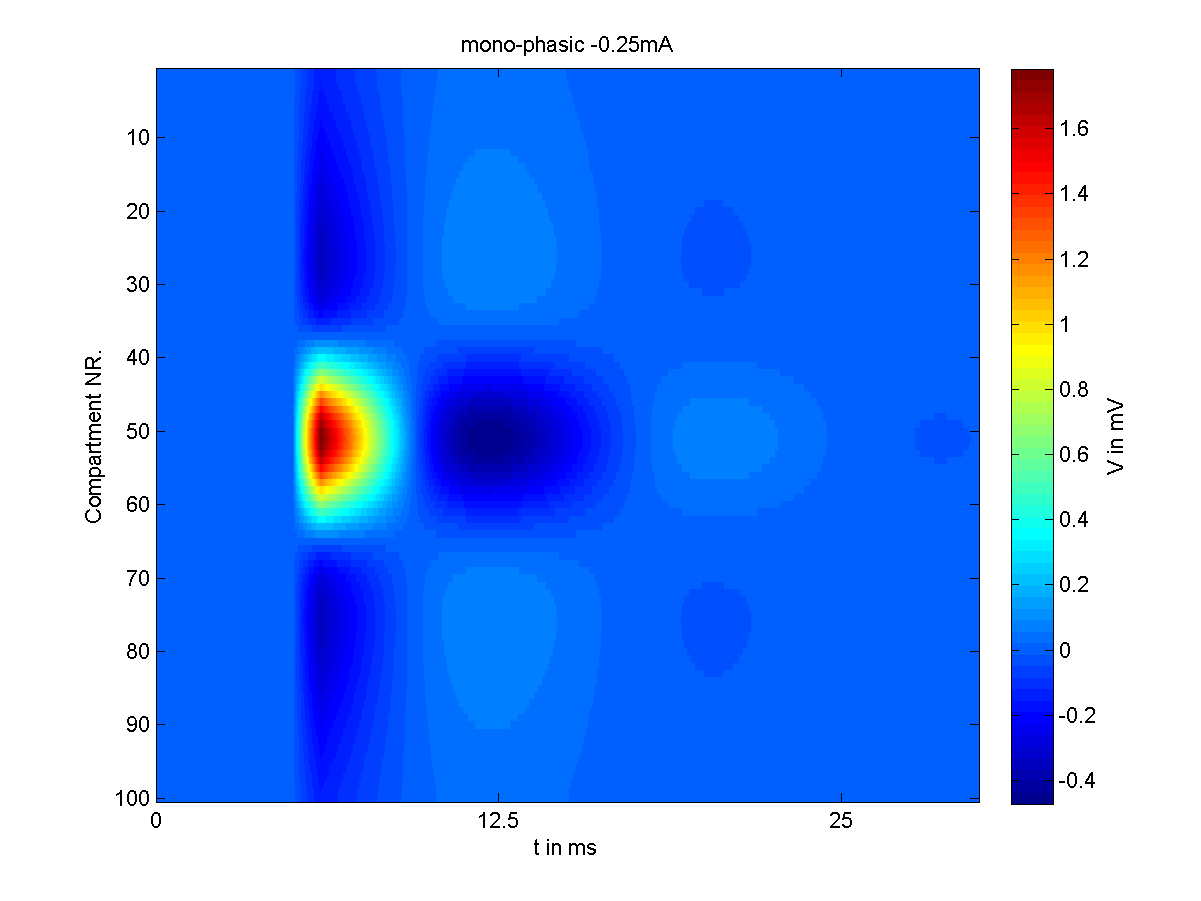
\includegraphics[width=0.5\textwidth]{img/mono_neg_025_1.png}
	\caption{Membranspannung mit I = -0.25mA (einphasig)}
	\label{fig:mono_neg_025_1}
\end{figure}

\item Einphasiger Strompuls mit Amplitude -1mA\\ (vgl. Abb. \ref{fig:mono_neg_1_1}) Da es sich hier auch um einen negativen Strom handelt, hat die Aktivierungsfunktion auch ihr Hauptmaximum in der Mitte (bei 0\textmu m bzw. bei Compartment 50). Der Strom ist groß genug, um eine Aktivierung zu erzeugen, die ein Aktionspotential hervorruft. Dieses propagiert symmetrisch nach links und rechts.
\begin{figure}[h!]
	\centering
	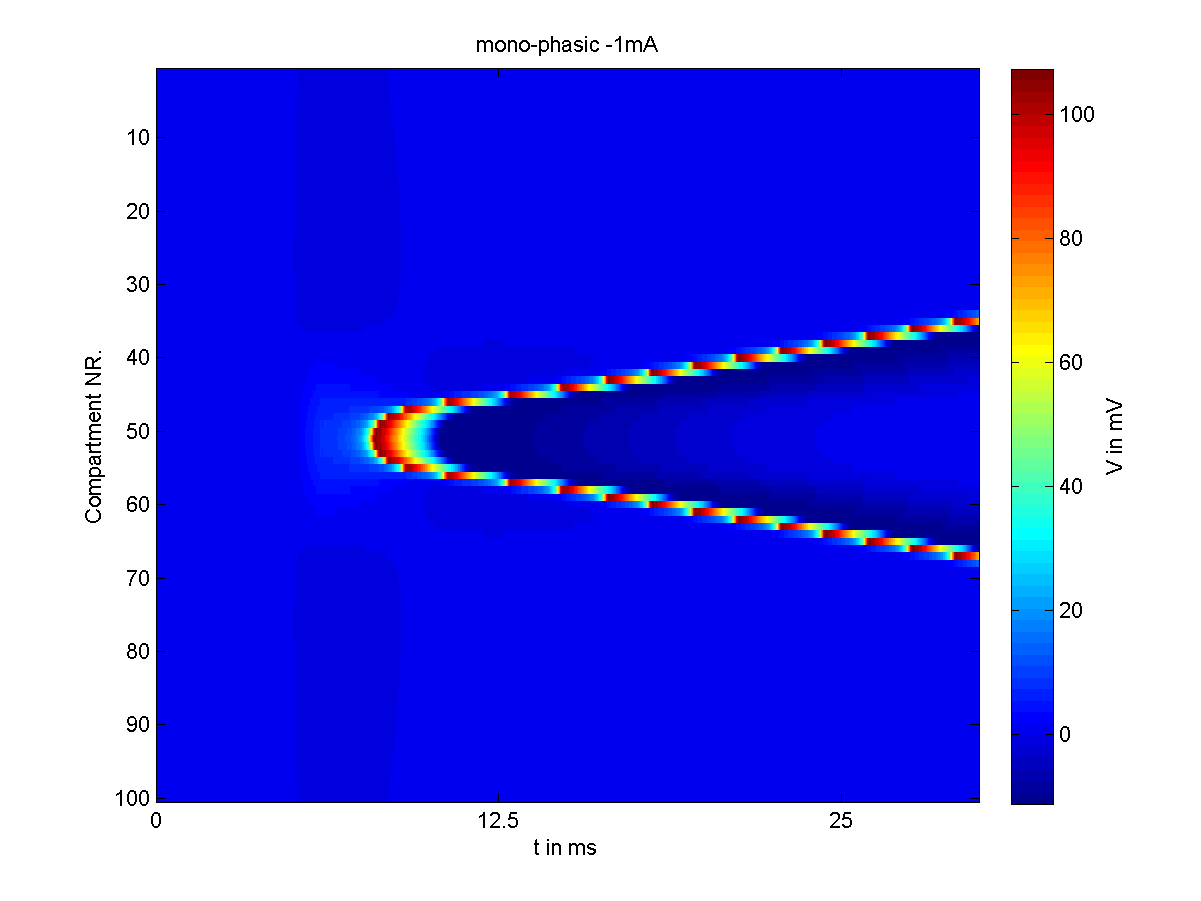
\includegraphics[width=0.5\textwidth]{img/mono_neg_1_1.png}
	\caption{Membranspannung mit I = -1mA (einphasig)}
	\label{fig:mono_neg_1_1}
\end{figure}

\item Bi-phasiger Strompuls mit Amplitude 0.5mA\\ (vgl. Abb. \ref{fig:bi_05_1}) Beim bi-phasigen Stromimpuls reicht auch eine Amplitude von 0.5mA noch nicht aus um ein Aktionspotential zu erzeugen. Vermutlich kommt dies daher, dass der zweite (gegenphasige) Strompuls dem ersten entgegenwirkt und die Aktivierung wieder verkleinert. Man kann jedoch nach dem positiven Puls schon erste Anzeichen eine Rebounds erkennen, da hier das Membranpotential nach der negativen Akivierungsfunktion leicht über den Ruhezustand hinausgeht.
\begin{figure}[h!]
	\centering
	\vspace{-10pt}
	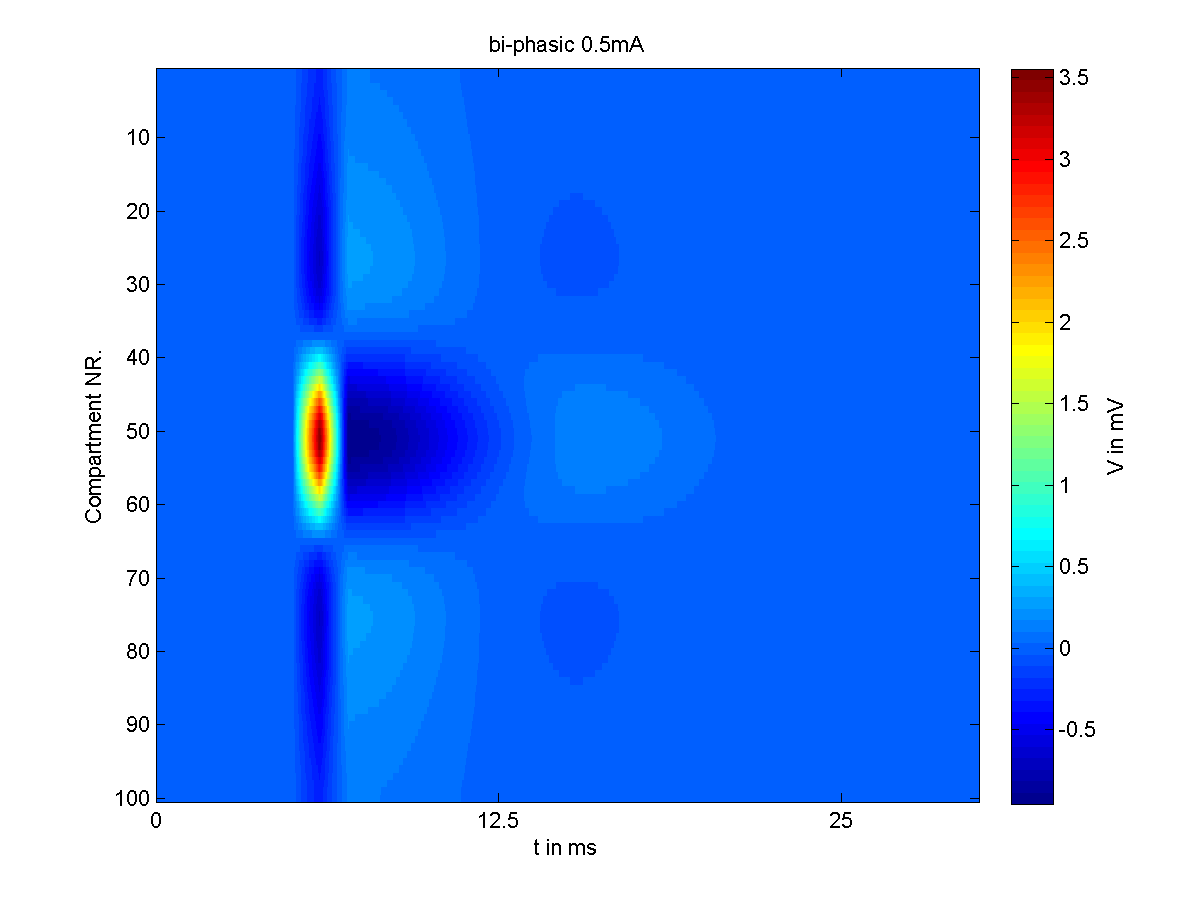
\includegraphics[width=0.5\textwidth]{img/bi_05_1.png}
	\vspace{-30pt}
	\caption{Membranspannung mit I = 0.5mA (bi-phasig)}
	\vspace{-5pt}
	\label{fig:bi_05_1}
	
\end{figure}

\item Bi-phasiger Strompuls mit Amplitude 2mA\\ (vgl. Abb. \ref{fig:bi_2_1}) Beim bi-phasigen Stromimpuls mit einer Amplitude von 2mA ist die Aktivierung so groß, dass ein Aktionspotential ausgelöst wird, welches dann wie in Fall 2 nach links und rechts propagiert. Auch der darauffolgende entgegengesetzt gepolte Strompuls kann das Aktionspotential nicht mehr aufhalten. Die zell-internen Ströme sind zu diesem Zeitpunkt schon so stark, dass kaum mehr ein hemmender Einfluss des positiven Stromes (negative Aktivierung) zu erkennen ist.
\begin{figure}[h!]
	\centering
	\vspace{-10pt}
	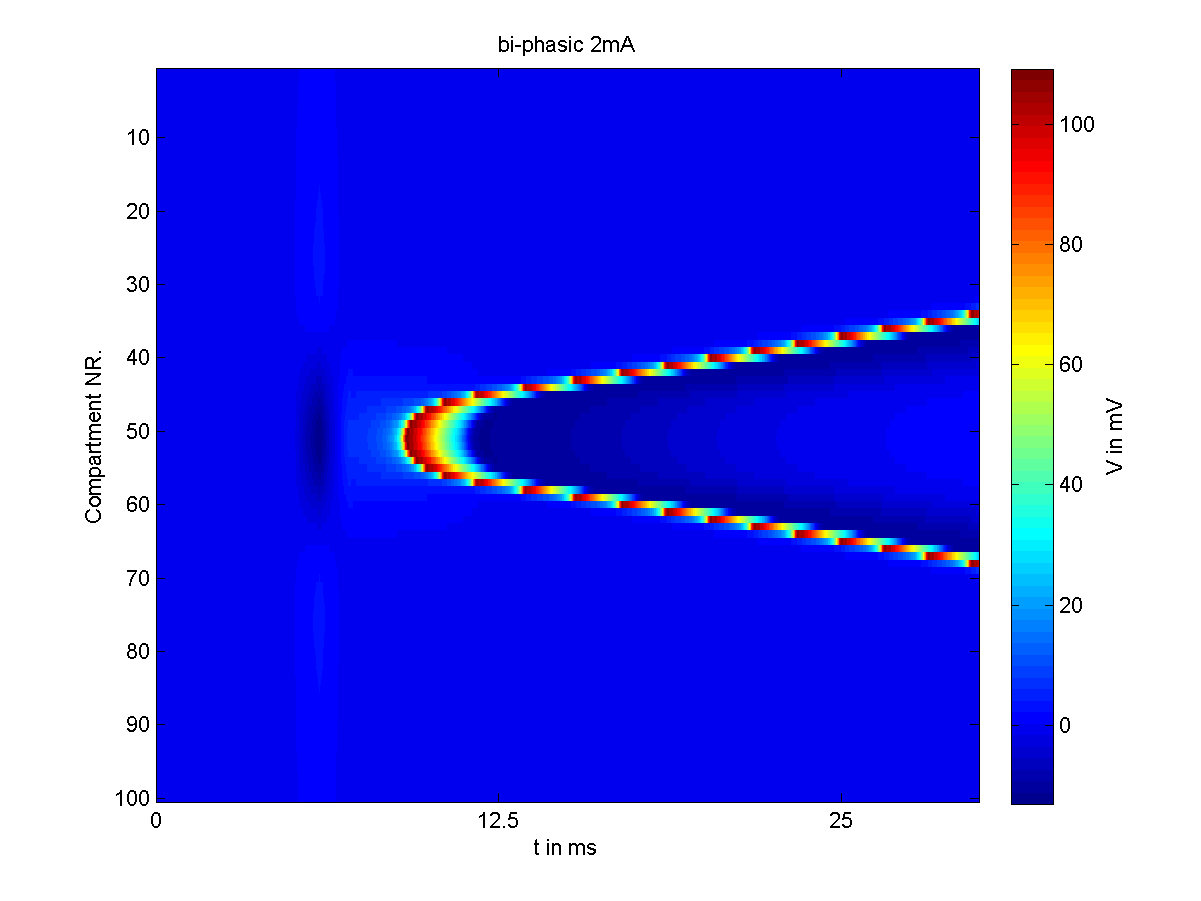
\includegraphics[width=0.5\textwidth]{img/bi_2_1.png}
	\vspace{-30pt}
	\caption{Membranspannung mit I = 2mA (bi-phasig)}
	\vspace{-5pt}
	\label{fig:bi_2_1}
\end{figure}

\item Einphasiger Strompuls mit Amplitude 0.25mA\\ (vgl. Abb. \ref{fig:mono_pos_025_1}) Der positive Strom Impuls verursacht eine Aktivierung mit einem negativen Hauptausschlag und zwei positiven Nebenmaxima (siehe Abb. \ref{fig:A1}). Weder der Rebound, noch die positiven Nebenmaxima sind groß genug um ein Aktionspotential auszulösen.
\begin{figure}[h!]
	\centering
	\vspace{-10pt}
	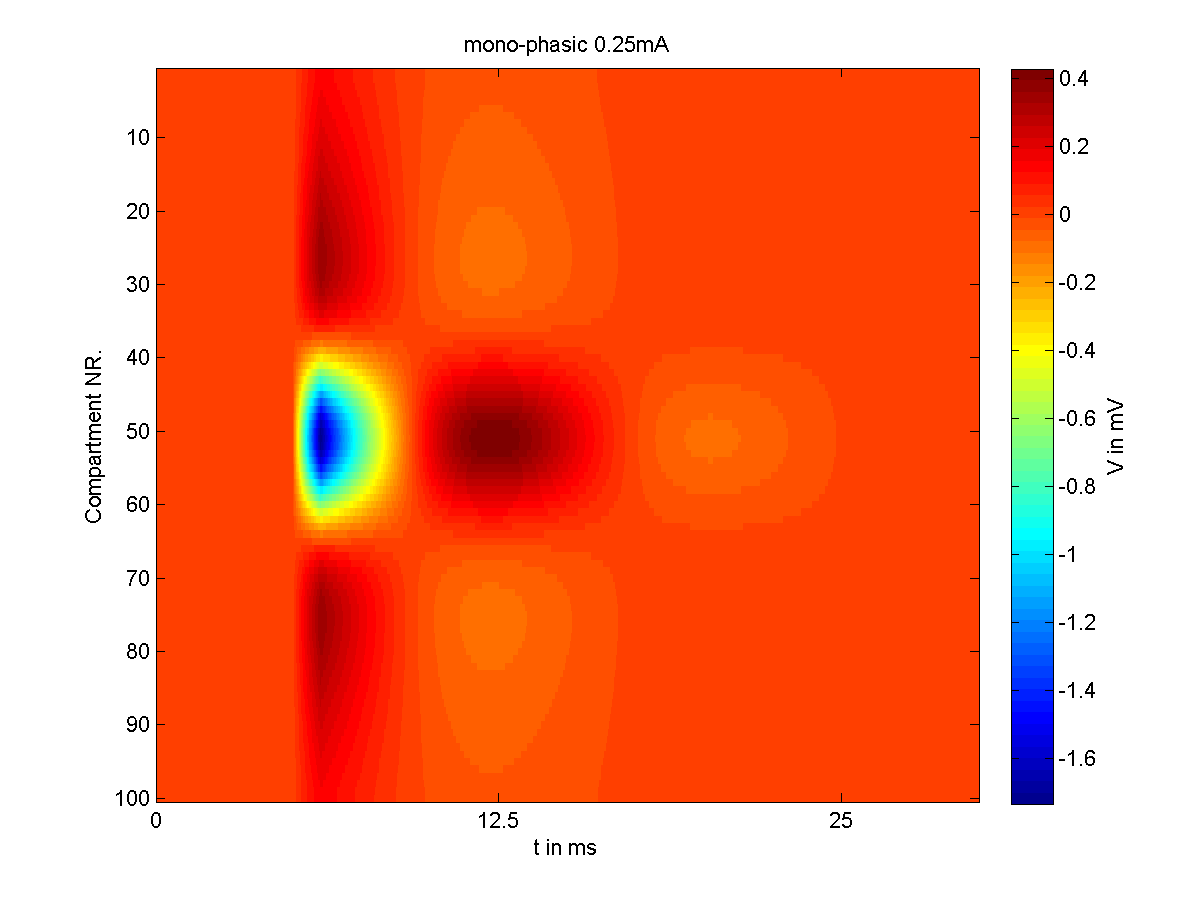
\includegraphics[width=0.5\textwidth]{img/mono_pos_025_1.png}
	\vspace{-30pt}
	\caption{Membranspannung mit I = 0.25mA (einphasig)}
	\vspace{-5pt}
	\label{fig:mono_pos_025_1}
\end{figure}

\item Einphasiger Strompuls mit Amplitude 5mA\\ (vgl. Abb. \ref{fig:mono_pos_5_1}) Beim positiven Strom mit Amplitude 5mA passieren zwei Dinge. Die Nebenmaxima sind so groß, dass diese an zwei stellen ein Aktionspotential auslösen. Diese propagieren jeweils nach innen und außen und würden sich in der Mitte treffen und gegenseitig wieder ausbremsen. Durch die extrem große negative Hauptamplitude der Aktivierungsfunktion kommt es auf dem Weg zur Rückkehr in den Ruhezustand zu einen Überschwingen durch den schnellen Natrium Strom. Der Kalium Strom ist langsamer und kann den Natrium Strom nicht so schnell ausgleichen, sodass es zu einem positiven Umschlag der Membranspannung kommt. Dies bezeichnet man auch als Rebound-Firing. Diese Mechanismus verursacht einige Millisekunden ein Aktionspotential in der Compartments in der Mitte des Axons. Dieses Aktionspotential propagiert jetzt als drittes durch das Axon und trifft auf die zur Mitte hin wandernden Teile der vorher ausgelösten Aktionspotentiale. Da ein Compartment einige Zeit nach einen Aktionspotential kein weiteres weiterlernten kann, da sie sich im refraktären Zustand befindet heben Aktionspotentiale auf, wenn sie aufeinander treffen. 
\begin{figure}[h!]
	\centering
	\vspace{-10pt}
	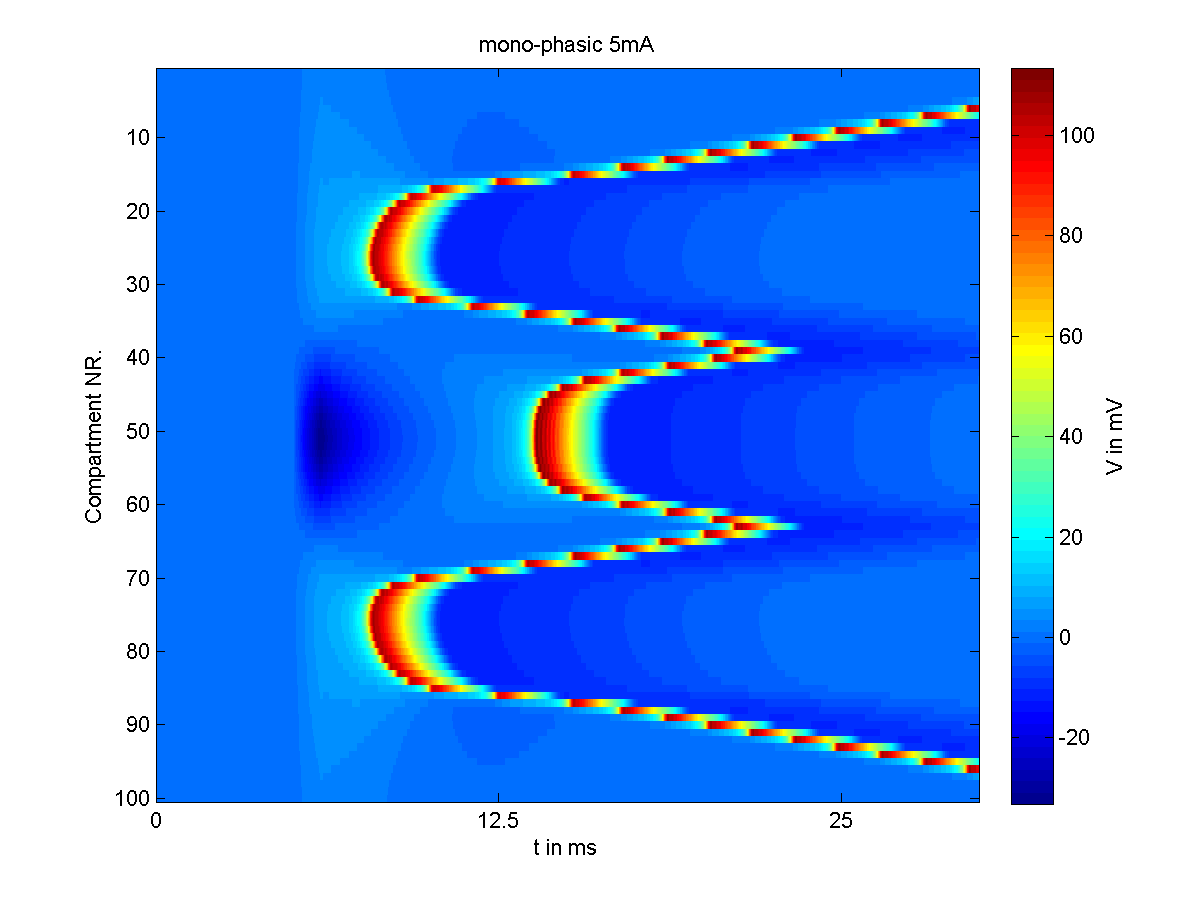
\includegraphics[width=0.5\textwidth]{img/mono_pos_5_1.png}
	\vspace{-30pt}
	\caption{Membranspannung mit I = 5mA (einphasig)}
	\vspace{-10pt}
	\label{fig:mono_pos_5_1}
\end{figure}

\end{enumerate}

\end{document}


